% Options for packages loaded elsewhere
\PassOptionsToPackage{unicode}{hyperref}
\PassOptionsToPackage{hyphens}{url}
%
\documentclass[
]{article}
\usepackage{amsmath,amssymb}
\usepackage{lmodern}
\usepackage{ifxetex,ifluatex}
\ifnum 0\ifxetex 1\fi\ifluatex 1\fi=0 % if pdftex
  \usepackage[T1]{fontenc}
  \usepackage[utf8]{inputenc}
  \usepackage{textcomp} % provide euro and other symbols
\else % if luatex or xetex
  \usepackage{unicode-math}
  \defaultfontfeatures{Scale=MatchLowercase}
  \defaultfontfeatures[\rmfamily]{Ligatures=TeX,Scale=1}
\fi
% Use upquote if available, for straight quotes in verbatim environments
\IfFileExists{upquote.sty}{\usepackage{upquote}}{}
\IfFileExists{microtype.sty}{% use microtype if available
  \usepackage[]{microtype}
  \UseMicrotypeSet[protrusion]{basicmath} % disable protrusion for tt fonts
}{}
\makeatletter
\@ifundefined{KOMAClassName}{% if non-KOMA class
  \IfFileExists{parskip.sty}{%
    \usepackage{parskip}
  }{% else
    \setlength{\parindent}{0pt}
    \setlength{\parskip}{6pt plus 2pt minus 1pt}}
}{% if KOMA class
  \KOMAoptions{parskip=half}}
\makeatother
\usepackage{xcolor}
\IfFileExists{xurl.sty}{\usepackage{xurl}}{} % add URL line breaks if available
\IfFileExists{bookmark.sty}{\usepackage{bookmark}}{\usepackage{hyperref}}
\hypersetup{
  pdftitle={Estimation of all-cause excess mortality by age-specific mortality patterns of COVID-19 pandemic in Peru in 2020},
  pdfauthor={Peter Lloyd-Sherlock; Ramón Martínez; Shah Ebrahim; Martin McKee; Enrique Acosta; Lucas Sempé},
  hidelinks,
  pdfcreator={LaTeX via pandoc}}
\urlstyle{same} % disable monospaced font for URLs
\usepackage[margin=1in]{geometry}
\usepackage{longtable,booktabs,array}
\usepackage{calc} % for calculating minipage widths
% Correct order of tables after \paragraph or \subparagraph
\usepackage{etoolbox}
\makeatletter
\patchcmd\longtable{\par}{\if@noskipsec\mbox{}\fi\par}{}{}
\makeatother
% Allow footnotes in longtable head/foot
\IfFileExists{footnotehyper.sty}{\usepackage{footnotehyper}}{\usepackage{footnote}}
\makesavenoteenv{longtable}
\usepackage{graphicx}
\makeatletter
\def\maxwidth{\ifdim\Gin@nat@width>\linewidth\linewidth\else\Gin@nat@width\fi}
\def\maxheight{\ifdim\Gin@nat@height>\textheight\textheight\else\Gin@nat@height\fi}
\makeatother
% Scale images if necessary, so that they will not overflow the page
% margins by default, and it is still possible to overwrite the defaults
% using explicit options in \includegraphics[width, height, ...]{}
\setkeys{Gin}{width=\maxwidth,height=\maxheight,keepaspectratio}
% Set default figure placement to htbp
\makeatletter
\def\fps@figure{htbp}
\makeatother
\setlength{\emergencystretch}{3em} % prevent overfull lines
\providecommand{\tightlist}{%
  \setlength{\itemsep}{0pt}\setlength{\parskip}{0pt}}
\setcounter{secnumdepth}{5}
\ifluatex
  \usepackage{selnolig}  % disable illegal ligatures
\fi
\newlength{\cslhangindent}
\setlength{\cslhangindent}{1.5em}
\newlength{\csllabelwidth}
\setlength{\csllabelwidth}{3em}
\newenvironment{CSLReferences}[2] % #1 hanging-ident, #2 entry spacing
 {% don't indent paragraphs
  \setlength{\parindent}{0pt}
  % turn on hanging indent if param 1 is 1
  \ifodd #1 \everypar{\setlength{\hangindent}{\cslhangindent}}\ignorespaces\fi
  % set entry spacing
  \ifnum #2 > 0
  \setlength{\parskip}{#2\baselineskip}
  \fi
 }%
 {}
\usepackage{calc}
\newcommand{\CSLBlock}[1]{#1\hfill\break}
\newcommand{\CSLLeftMargin}[1]{\parbox[t]{\csllabelwidth}{#1}}
\newcommand{\CSLRightInline}[1]{\parbox[t]{\linewidth - \csllabelwidth}{#1}\break}
\newcommand{\CSLIndent}[1]{\hspace{\cslhangindent}#1}

\title{Estimation of all-cause excess mortality by age-specific mortality patterns of COVID-19 pandemic in Peru in 2020}
\author{Peter Lloyd-Sherlock\footnote{University of East Anglia} \and Ramón Martínez\footnote{Pan American Health Organisation} \and Shah Ebrahim\footnote{London School of Hygiene and Tropical Medicine} \and Martin McKee\footnote{London School of Hygiene and Tropical Medicine} \and Enrique Acosta\footnote{Max Planck Institute for Demographich Research} \and Lucas Sempé\footnote{University of East Anglia - email:\href{mailto:l.sempe@uea.ac.uk}{\nolinkurl{l.sempe@uea.ac.uk}}}}
\date{28 May 2021}

\begin{document}
\maketitle

\hypertarget{summary}{%
\section*{Summary}\label{summary}}
\addcontentsline{toc}{section}{Summary}

\hypertarget{background}{%
\subsection*{Background}\label{background}}
\addcontentsline{toc}{subsection}{Background}

All-cause excess mortality is a comprehensive measure of the combined direct and indirect effects of COVID-19 on mortality. Estimates are usually derived from Civil Registration and Vital Statistics (CRVS) systems, but these do not include non-registered deaths, which may be affected by changes in vital registration coverage over time.

\hypertarget{methods}{%
\subsection*{Methods}\label{methods}}
\addcontentsline{toc}{subsection}{Methods}

We use quasi-Poisson models to estimate excess registered mortality in Peru during the first wave of the COVID-19 pandemic during 2020. We use logistic mixed-effects models to estimate the completeness of the new online registration system (SINADEF) at this time.

\hypertarget{findings}{%
\subsection*{Findings}\label{findings}}
\addcontentsline{toc}{subsection}{Findings}

We estimate that registered mortality nationally underestimates mortality by 24.6\% (95\% CI 48.1\% - 20.9\%). We estimate total all-cause excess mortality during the period of analysis at 117,574 (95\% CI 114,101 - 139,810) of which 94,373 (95\% CI 79,139 - 105,767) were captured by the vital registration system. Deaths at age 60 and over accounted for 75.4\% (95\% CI 75.7\% - 75.4\%) of total excess deaths, while there were fewer deaths than expected in younger age groups. Lima region, on the Pacific coast and including the national capital, accounts for 61,986 (95\% CI 61,918 - 69,672) excess deaths, while the regions of Madre De Dios and Pasco account for less than 100 excess deaths.

\hypertarget{interpretation}{%
\subsection*{Interpretation}\label{interpretation}}
\addcontentsline{toc}{subsection}{Interpretation}

Estimating excess mortality in low- and middle-income countries (LMICs) such as Peru must take under-registration of mortality into account. Combining demographic trends with data from administrative registries reduces uncertainty and measurement errors. In countries like Peru, this is likely to produce significantly higher estimates of excess mortality than studies that do not take these effects into account.

\hypertarget{funding}{%
\subsection*{Funding}\label{funding}}
\addcontentsline{toc}{subsection}{Funding}

None.

\hypertarget{research-in-context}{%
\section*{Research in context}\label{research-in-context}}
\addcontentsline{toc}{section}{Research in context}

\hypertarget{evidence-before-this-study}{%
\subsection*{Evidence before this study}\label{evidence-before-this-study}}
\addcontentsline{toc}{subsection}{Evidence before this study}

We searched PubMed, Google Scholar, medRxiv, and SocArXiv for studies published up to May 27, 2020, using the key words ``excess mortality'' and ``under-registration'' or ``subregistration,'' combined with ``coronavirus'' or ``SARS-CoV-2'' or ``COVID-19.'' We found studies estimating cumulative mortality in high-income countries in Europe and North America solely based on official death counts. We found studies computing overall COVID-19 mortality for a small number of LMICs. Prior research shows a significant percentage of under-registration of deaths in LMICs.

\hypertarget{added-value-of-this-study}{%
\subsection*{Added value of this study}\label{added-value-of-this-study}}
\addcontentsline{toc}{subsection}{Added value of this study}

To our knowledge, we provide the first estimate of excess mortality associated with COVID-19 in a LMIC accounting for both registered and unregistered deaths. We develop an analytical strategy to address common challenges faced by LMICs, such as low completion rates of death certificates, missing data, vital registration growth, and inconsistency and variability of data across regions and age groups.

\hypertarget{implications-of-all-the-available-evidence}{%
\subsection*{Implications of all the available evidence}\label{implications-of-all-the-available-evidence}}
\addcontentsline{toc}{subsection}{Implications of all the available evidence}

Our approach shows the importance of accounting for unregistered deaths based on demographic trends to generate robust estimates of excess mortality associated with COVID-19. It suggests that previous reports of COVID-19 related mortality in Peru were substantial underestimates.

\hypertarget{introduction}{%
\section{Introduction}\label{introduction}}

Monitoring mortality is an essential part of the public health response to the COVID-19 pandemic. In many countries, accurate COVID-19 mortality monitoring has been hindered by failure to capture all deaths and to attribute causes of deaths to those that are recorded.\textsuperscript{1} Disentangling the contribution of COVID-19 to overall mortality is especially challenging, as many people who die from COVID-19 have other conditions, such as cardiovascular disease and diabetes.\textsuperscript{2} A further complication is the decision of some countries to apply an arbitrary maximum cut-off time between a positive COVID-19 test and death when deciding whether to attribute mortality to this cause.\textsuperscript{3} Also, it is widely documented that the pandemic has led to large numbers of deaths not directly attributable to COVID-19 (either exclusively or in part), due to the wider impacts of responses, including reduced access to treatment for other conditions.\textsuperscript{4,5} Conversely, there is evidence that the pandemic has, to a limited extent, reduced expected rates of mortality from causes such as road traffic injuries and homicides during lockdowns.\textsuperscript{6}

In the absence of good data on these different mortality effects, robust estimation of all-cause excess mortality offers the most complete and reliable approach for gauging the overall impact of the pandemic on mortality in a defined population over a fixed period of time.\textsuperscript{7} Excess mortality refers to the number of additional deaths occurring over a time period when specific conditions apply (in this case, the presence of COVID-19), compared to the number of deaths we might reasonably expect over the same period based on historical data. It captures deaths directly and indirectly attributed to COVID-19 and corresponding responses, to provide an estimate of the overall mortality effect of the pandemic as it unfolds.\textsuperscript{8}

Excess mortality estimates have been computed for high-income countries based on registered deaths by surveillance agencies\textsuperscript{9,10}, academia\textsuperscript{11--14} and news agencies.\textsuperscript{15--18} However, these types of data are often incomplete or inaccurate, especially in many low and middle-income countries (LMICs). The Global Burden Disease (GBD) project estimates that only 64\% of global deaths were registered in 2015.\textsuperscript{19} In most LMICs, responsibility for mortality data is often divided between different national and subnational agencies.\textsuperscript{20} This can cause extended delays in national reporting and discrepancies between different sources.\textsuperscript{12,21} Disaggregation of summary data by different geographical areas or demographic groups is usually very limited.\textsuperscript{22} These shortcomings in mortality data explain a lack of published studies of excess mortality in LMICs.\textsuperscript{23,24}

We analyse excess mortality associated with the COVID-19 pandemic in Peru during 2020. This country is well-suited to our analytical approach. Like much of Latin America, Peru has experienced high levels of COVID-19 mortality. Official sources report 37,723 deaths directly caused by COVID-19 between 18 March and December 31 2020. However, these only include cases with positive COVID-19 test results and rates of testing in Peru have been low compared to other Latin American countries.\textsuperscript{25} Also, many tests have used low sensitivity devices, potentially generating false negatives.\textsuperscript{26} On the other hand, Peru does place anonymised individual level data on mortality and COVID-19 in the public domain.\textsuperscript{27} Other studies show that unregistered mortality tends to be more prevalent among older people and in poorer regions.\textsuperscript{28,29} However, as in many LMICs, Peru does not report under registration for sub-national data or disaggregated by age.

Potentially, our analytical design could be applied to other countries where mortality registration and cause of death data are incomplete. It may offer a valuable contribution towards assessing the true global impact of the COVID-19 pandemic.

\hypertarget{data-and-methods}{%
\section{Data and methods}\label{data-and-methods}}

\hypertarget{data}{%
\subsection{Data}\label{data}}

We combine several demographic data sources to forecast mortality rates. These sources are (i) population projections from Peru's National Institute of Statistics and Information (INEI, for its acronym in Spanish) for 2020 disaggregated by region and age group (the most recent census was in 2017); (ii) crude mortality rate estimates disaggregated by region and year from 2015 to 2020 from INEI; (iii) individual-level registered COVID-19 deaths by region and age in 2020 from the Ministry of Health (MoH); and, (iv) individual-level registered deaths by region and age since 2017 from the National electronic registration of deaths system (SINADEF, for its acronym in Spanish). SINADEF registers individual-level data since 2017 with a progressive although still unequal among regions,\textsuperscript{27} which enables comparisons of spatial and temporal trends in death registration in the country.

\hypertarget{excess-mortality-methods}{%
\subsection{Excess mortality methods}\label{excess-mortality-methods}}

Figure \ref{fig:conceptual} represents our approach to estimate excess mortality, which can be decomposed into four terms: (i) SINADEF registration growth rateS (ii) excess registered deaths; (iii) excess unregistered deaths; and, (iv) unregistered COVID-19 deaths. While the terms (ii)-(iv) add counts towards the final estimation of total excess deaths, the first term adjusts downwards the final estimation. Although terms (i) and (iii) could be understood as a similar phenomeno, they are distingued based on post and pre pandemic wave, respectively.

\begin{center}
  [FIGURE \\ref{fig:conceptual} ABOUT HERE]
\end{center}

Figure \ref{fig:model} summarises data sources used (squares), analysis performed (diamonds) and different outputs (circles).

\begin{center}
  [FIGURE \\ref{fig:model} ABOUT HERE]
\end{center}

The first term, SINADEF registration growth rate, \(\widehat{\mu}_{\text{Registration}_\text{Growth}}\) is computed for each region by comparing the average mortality during the period previous and post first wave. We determine the starting and ending points calculating the increment in the percentage from one weeks to the next one\textsuperscript{30} fixing 0.60\% as criterion of change and assuming a linear registration growth rate during the first wave, as follows:

\begin{equation}
\label{eq:reggrowth}
   \begin{aligned}
  \widehat{\mu}_{\text{Registration}_\text{Growth}} = \big(1-(\hat\mu_{Deaths_{Post}}-\hat\mu_{Deaths_{Pre}}/\hat\mu_{Deaths_{Pre}}*0.5)\big)
   \end{aligned}      
\end{equation}

To estimate the second term, excess registered deaths, we rely on data from SINADEF. Due to the overdispersed and count nature of data, we fit quasi-Poisson regressions to weekly deaths by age-groups and region, as follows:

\begin{equation}
  \label{eq:registered}
  \begin{aligned}
  log(\text{Deaths}_{i})=\beta_0+\beta_1\text{COVID-19}+\beta_2\epsilon_{t-1}+
  \sum\beta_k\phi_{k}(\text{Week})+
  \text{log}(\text{Pop})+\epsilon_{t}
   \end{aligned}  
\end{equation}

where we fit a natural cubic B-spline function \(\phi_{k}(\text{Week})\) on weeks to address long-term trends and seasonality.\textsuperscript{31} Additionally, we use lagged residuals \(\epsilon_{t-1}\) and the log of population in 2020 as an offset. Finally, we compute a dichotomous variable \(\text{COVID-19}\) starting in the week corresponding to March 15 2020 as the first registered death of COVID-19 in the country.

Then we compute the excess registered mortality as a population attributable fraction (PAF)\textsuperscript{32} based on the relative risk \(\text{RR}\) from parameter \(\beta_1\) in equation \eqref{eq:registered}, as follows:

\begin{equation}
\label{eq:rr}
\begin{aligned}
\widehat{{\text{Excess}}_\text{Reg}} = (\text{RR}-1)/\text{RR}*\text{n}
\end{aligned}
\end{equation}

where \(\text{n}\) is the weekly number of deaths,\textsuperscript{33} and represents a fraction of the total mortality of the period where \(\text{COVID-19}=1\) in equation \eqref{eq:registered}.

\textbf{\emph{The subsequent prediction of completeness from model (3) would benefit from additional explanation. How is completeness defined?}}

The third term, excess unregistered deaths, is computed as a fraction of \(\widehat{{\text{Excess}}_\text{Reg}}\) based on the completeness of SINADEF previous to 2020. We start by predicting the random-effects logit regressions of SINADEF completeness \(\text{Reg complete}\) for each region \(\text_{j}\)\textsuperscript{29} using data from 2017 and 2019. We exploit variability in INEI mortality rates, population aged 60 years and over and rurality to address potential differences in terms of registration completeness, using the equation:

\begin{equation}
\label{eq:adair}
\begin{aligned}
  \text{logit}(\text{Reg complete}_{j})=
  \beta_0+
  \beta_1*\text{RegCDR}+
  \beta_2*\text{RegCDR}^2+\\
  \beta_3*\text{complete < 5}+
  \beta_4*\text{P}_{60+}+
  \beta_5*\text{log}(\text{5q0})+ 
  \beta_6*\text{LPG} +
  \beta_7*\text{Year}+
  \epsilon + 
  \gamma_{j}
\end{aligned}
\end{equation}

where \(\text{RegCDR}\) and \(\text{RegCDR}^2\) are the Crude Death Rates, \(\text{complete < 5}\) is the completeness registration rate for infants, \(log(\text{5q0})\) is the logarithm under-five mortality rate and \(\text{P}_{60+}\) represents the fraction of the population at 60 years and over based on INEI projections. \(\text{LPG}\) is the share of households that use liquefied petroleum gas (LPG) for cooking, which is an acceptable proxy for rurality in Peru, where 81.8\% of rural households primarily use solid fuel compared to 9.8\% of urban households, who typically cook with LPG.\textsuperscript{34} Rurality is an important factor to explain delays and under registration of deaths as the system requires access to internet and computers. Additionally, \(\epsilon\) in the error term and \(\gamma_{j}\) is the region-level random effect. \(\text{Reg complete}_{j}\) is computed using the inverse logit of the predicted values, which provides a regional adjusted SINADEF completeness rate.

Finally, the term excess unregistered deaths, \(\widehat{{\text{Excess}}_\text{Reg}}\), is computed based on \(\text{Reg complete}_{j}\) and \(\widehat{\mu}_{\text{Registration}_\text{Growth}}\) from equation \eqref{eq:reggrowth}, as follows:

\begin{equation}
\label{eq:unreg}
  \begin{aligned}
  \widehat{\mu}_{\text{Deaths}_\text{Not reg}}=\sum{\widehat{{\text{Excess}}_\text{Reg}}} * \big(1-\widehat{\text{Completeness}}\big) * \big(1-\widehat{\mu}_{\text{Registration}_\text{Growth}}\big)
   \end{aligned}      
\end{equation}

The last term, unregistered COVID-19 deaths, is computed to correct for situations where the proportion of cumulative cases of COVID-19 exceeds registered deaths for that period, base on MoH Covid-19 database. It follows a deterministic approach conditional on excess registered deaths being lower than officially registered COVID-19 deaths for each region and specific age-group as follows:

\begin{equation}
\label{eq:covidnotreg}
   \widehat{\mu}_{\text{Deaths}_\text{COVID not reg}}=  
   \begin{cases}
    \begin{aligned}
 &  \widehat{\mu}_{\text{Deaths}_\text{COVID Reg}}-\widehat{\mu}_{\text{Excess}_\text{Reg}} \; & \text{if }\widehat{\mu}_{\text{Deaths}_\text{COVID Reg}} > \widehat{\mu}_{\text{Excess}_\text{Reg}},\\[1ex]
& 0 \;& \text{if }\widehat{\mu}_{\text{Deaths}_\text{COVID Reg}} < \widehat{\mu}_{\text{Excess}_\text{Reg}}.
  \end{aligned}
    \end{cases} 
\end{equation}

Finally, we estimate total excess deaths for different scenarios.

A first scenario is when there is no solid evidence suggesting under-registration of deaths for some regions or age groups and, therefore, no scope to expand registration over time. This usually occurs in areas and age groups with very small populations. In those cases \(\widehat{\mu}_{\text{Deaths}_\text{Not reg}}\) is set to 0 as, if not, they would add negative values to the sum. A second scenario is related to younger age groups in some regions that have not be significantly affected by COVID-19 mortality. This case corresponds to when \({\beta_{1}}\) in equation \eqref{eq:registered} is not statistically significant and therefore we set \(\widehat{{\text{Excess}}_\text{Reg}} = 0\). A third scenario is when some groups have fewer deaths than expected, due to effects such as reduced road traffic injuries caused by lockdowns. In these groups \(\widehat{{\text{Excess}}_\text{Reg}}\le 0\) and
\(\widehat{\mu}_{\text{Deaths}_\text{Not reg}} = 0\) are taken account of in our final estimation. A fourth scenario is when models underestimate the official number of deaths such as \(\text{COVID Reg} > \widehat{{\text{Excess}}_\text{Reg}}\). In this case, we use the first as registered deaths. Equation \eqref{eq:finale} summarises the estimation of \(\widehat{\text{Excess}}_{\text{T}_{\text{min/mean/max}}}\) as follows:

\begin{equation}
\label{eq:finale}
  \begin{aligned}
    \widehat{\text{Excess}}_{\text{T}_{\text{min/mean/max}}} =
      \widehat{{\text{Excess}}_\text{Reg}}_{\text{min/mean/max}}  +   
        \widehat{\mu}_{\text{Deaths}_\text{Not reg}}
         +{\text{Deaths}_\text{COVID Not Reg}} 
  \end{aligned}
\end{equation}

Finally, we estimate total mortality during 2020 by adding \(\widehat{\text{Excess}}_{\text{T}_{\text{min/mean/max}}}\) from equation \eqref{eq:finale} and the counterfactual difference of SINADEF deaths during 2020 and \(\widehat{{\text{Excess}}_\text{Reg}}_{\text{min/mean/max}}\), adjusted by \(\widehat{\text{Completeness}}\) as follows:

\begin{equation}
\label{eq:totalmort}
        \begin{aligned}
    \widehat{\text{Total}_{Mortality \ 2020}}=\widehat{\text{Excess}}_{\text{T}_{\text{min/mean/max}}}+\Big(\big(\sum\limits_{week=1}^{52}\text{SINADEF}_{2020}-
    \widehat{{\text{Excess}}_\text{Reg}}_{\text{min/mean/max}}\big)*\big(1+\widehat{\text{Completeness}}\big)\Big)
    \end{aligned} 
\end{equation}

To address the relative magnitude of mortality in 2020, we compute all cause age-standardised death rates per 1,000 people derived from the estimated total excess deaths. We use the direct standardization methods\textsuperscript{35} based on population INEI population estimates by region and age-group for 2020 as the standard population.\textsuperscript{36}

As a robustness check for excess mortality estimates, we estimated a mortality baseline for each age group fitting a Generalised Linear Model with Poisson or Negative binomial distributions, depending on the data's overdispersion. The model includes natural splines and sinusoidal components to account for secular changes and seasonality in mortality, as well as interpolated weekly exposures to control for changes in age structure over time. 95\% prediction intervals were estimated using 2,000 bootstrapping iterations. Excess mortality is computed as the difference between observed mortality and the baseline, only including weeks in which observed mortality was above the upper prediction interval.

\hypertarget{results}{%
\section{Results}\label{results}}

Figure \ref{fig:trend} shows weekly deaths registered during years 2017-2020 where dotted vertical lines signaling start and end estimated points of the first pandemic wave. Those thresholds were used to compute the excess mortality period and the registration growth rate.

\begin{center}
[FIGURE \\ref{fig:trend} ABOUT HERE]
\end{center}

Estimates of completeness of registration derived from our logistic regression model fit the data according to marginal and conditional \(\text{R}^2\) and Root Mean Square of Errors parameters. Model fit and goodness-of-fit are presented in Appendix 1. Figure \ref{fig:map} shows important variations in regional completeness rates: Amazonas and Loreto (in Amazonia), Lambayeque (on the coast), and Cajamarca and Pasco (in the Andes) show estimated completion at below 40\%, while Ica (coast) and Madre De Dios (Peru's least populated regions in Amazonia) appear to have complete registration (see Appendix 1).

\begin{center}
[FIGURE \\ref{fig:map} ABOUT HERE]
\end{center}

Figure \ref{fig:growth}

\begin{center}
[FIGURE \\ref{fig:growth} ABOUT HERE]
\end{center}

Figure \ref{fig:predicted} shows predicted values for excess registered mortality for the age group over 80. The line fit

\begin{center}
        [FIGURE \\ref{fig:predicted} ABOUT HERE]
\end{center}

Table \ref{tab:summary} summarises our estimates of excess mortality. The quasi-Poisson models show a good fit for our first term (weekly excess registered deaths) across models. Excess registered mortality is estimated to be 94,373 ( 95\% CI 79,139 - 105,767 ), of which 37,725 are reported as COVID-19 deaths. This represents an increase of 150 \% ( 95\% CI 110 \% - 180 \%) compared to MoH data. See Appendix 2 for results and comparison with robustness analysis.

\begin{center}
[TABLE \\ref{tab:summary} ABOUT HERE]
\end{center}

Table \ref{tab:exineidepq} shows estimates by region. Lima, which includes the capital, accounts for 61986 ( 95\% CI 61918 - 69672 ) total excess deaths, and Madre De Dios and Pasco show the lowest numbers. Table \ref{tab:exineiageq} shows excess mortality estimates by age group. Deaths among people aged 60 years and over accounts for 75.4\% of total excess mortality. There was negative excess registered mortality for the youngest three age groups: under 10, 10 to 19 and 20 to 29.

\begin{center}

[TABLE \\ref{tab:exineidepq} ABOUT HERE]
        
\end{center}

\textbackslash end\{center\}

{[}TABLE \ref{tab:exineiageq} ABOUT HERE{]}

\textbackslash end\{center\}

Our second term, excess unregistered deaths, is estimated to be 14,780 deaths ( 95\% CI 25,622 - 26,541 ). This represents 19.7 \% ( 95\% CI 10 \% - 32.7 \%) of our estimate of the total registered and unregistered deaths. Coastal regions show the highest values where Lima accounts for 11,054 additional deaths, followed by Piura (4,631) and Lambayeque (1,512). Our third term adds 8,421 deaths corresponding to cases when reported COVID-19 deaths exceed our estimate of adjusted excess registered mortality. This mainly occurs for some smaller groups at younger ages. The regions with the highest under reported COVID-19 values are the Andean regions of Ayacucho (4,631), Cusco (794) and Puno (556).

Combining all these terms, our estimate of total excess deaths during 2020 is 117,574 ( 95\% CI 114,101 - 139,810 ) and our estimate of total deaths for 2020 is 278,499 ( 95\% CI 258,902 - 322,458 ). This is 0.3 \% ( 95\% CI -11.3 \% - 11 \%) more than the number of deaths projected by INEI for 2020.

Figure \ref{fig:map2} shows all cause age-standardised death rates. We find that Tumbes, Moquegua, and Lambayeque (CI 95\% ranging from 11.1 to 12.9) present the highest rates, ranging from 11.5 to 12.7, while regions of Amazonas, Ayacucho, and Cusco show the lowest rates ranging from 4.92 to 6.52 (CI 95\% ranging from 4.72 to 6.66) (left). Figure \ref{fig:map2} (right) shows differences deaths per 1000 in comparison to INEI's projections for 2020. We find excess mortality rates in all cases but Amazonas, which shows -1.26 suggesting that INEI overestimates mortality rates projections for 2020 and there is lower use of the CRVS system than expected.

\begin{center}
[FIGURE \\ref{fig:map2} ABOUT HERE]
\end{center}

\hypertarget{discussion}{%
\section{Discussion}\label{discussion}}

The COVID-19 pandemic has underscored the need for methodological advances in population health measurement, research, critical data quality assessment and improvement of health information systems to obtain reliable information on the impact of the pandemic from multiple data sources linked to COVID-19. In this regards, our study provides a framework, tools and analytical strategy to estimate the excess mortality caused by the COVID-19 pandemic in Peru and, potentially, other countries where the quality of mortality data is medium to low.\textsuperscript{37} The scope for applying a similar approach will vary between countries. In countries such as India, where mortality and cause of death data are of considerably lower quality than in Peru, achieving robust estimates by any method will be hugely challenging.\textsuperscript{38} In other countries, such as Colombia, data quality is similar to Peru's and a recent reform of its CRVS system is likely to have boosted registration rates in the past recent years.\textsuperscript{39}

Other published studies of excess COVID-19 mortality fall into two categories. Some studies provide estimates for countries where mortality data are relatively complete and reliable.\textsuperscript{40--43} As such, they do not apply specific methods to address data gaps. Studies of excess COVID-19 mortality for countries with less complete data do not take account of unregistered deaths.\textsuperscript{44--47}

We estimate that overall excess mortality in Peru was 212 \% ( 95\% CI 202 \% - 271 \%) higher than the level officially attributed to COVID-19. Registered excess mortality was 150 \% ( 95\% CI 110 \% - 180 \%) higher. This is a larger differential than reported by studies for high-income countries. For example, separate studies of the USA show differentials of between 28 and 33\%.\textsuperscript{11,12} Our estimates are higher than those previously published for Peru, which are only based on registered deaths, and which apply simpler methods.\textsuperscript{48,49} Our estimates of regional variations in excess mortality are in line with,\textsuperscript{48} who speculate that they may be in part attributable to the effect of altitude of COVID-19 case fatality.

Despite making up a relatively low share of Peru's population (12.5\% in 2020), people aged 60 or more accounted for 75.4\% of excess mortality. No other published study in Peru provides data disaggregated by age groups. A study of registered excess mortality in six Brazilian cities reports that people aged 60 and over accounted for 71.1\% of the total.\textsuperscript{45} An analysis of European countries reports that 91\% of excess COVID-19 deaths occurred among people aged 65 or more.\textsuperscript{42} This reflects a higher proportion of population aged 60 or more in Europe (25.5\% in 2020) than in Peru.

\hypertarget{limitations}{%
\section{Limitations}\label{limitations}}

Our analysis assumes that comparison between years is not invalidated by specific time-bound mortality events such as additional disease outbreaks or other major external shocks. Our estimates of registration completeness assume no variation across age groups, which may not be the case. We do not take into account changes in registration over time as our estimates are based on provisional data, which are incomplete and continue to be fatalities due to COVID-19. Finally, we present a conservative scenario, allowing for the existence of negative as well as positive excess deaths.

assuming a linear registration growth rate during the first wave

\hypertarget{conclusion}{%
\section{Conclusion}\label{conclusion}}

There is an evident need for robust estimates of the direct and indirect mortality effects of the COVID-19 pandemic. To date, much of the data for LMICs in the public domain rely on officially-registered deaths. Inaccurate attribution of cause of death can, to some degree, be resolved by generating excess mortality estimates based on temporal comparisons of all-cause mortality. Also, these approaches do not include deaths that are not officially registered. This paper develops and applies a method to obtain robust estimates of excess mortality for both registered and unregistered deaths.

Our study indicates that official data under-represent the overall mortality impact of the COVID-19 pandemic in Peru. This gap is considerably greater than those reported for high-income countries. It is plausible that under-estimation of excess mortality in other countries with low quality mortality data will be comparable to Peru. In that case, LMICs would account for a much larger share of the global distribution of excess mortality associated with the COVID-19 pandemic than indicated by official data sources.

\hypertarget{contributors}{%
\section{Contributors}\label{contributors}}

LS conceived and initiated the study, did the statistical analysis and visualisations and drafted the manuscript.

PLS conceived and supervised the study, drafted the manuscript and led the editing process of the manuscript.

MM and SE supervised the study and engaged in the draft review \& editing

RM contributed in the data curation and methodology process and reviewed \& edited the draft.

EA contributed in data curation, methodology and statistical analysis.

LS and EA had access to all the data. All authors approved the manuscript and are responsible for the decision to submit for publication.

\hypertarget{declaration-of-interests}{%
\section{Declaration of interests}\label{declaration-of-interests}}

RM is a staff member of the Pan American Health Organization. The author alone is responsible for the views expressed in this publication, and they do not necessarily represent the decisions or policies of the Pan American Health Organization.

All other authors declare no competing interests.

\hypertarget{data-sharing}{%
\section{Data sharing}\label{data-sharing}}

Data presented in this manuscript are made publicly available at \url{https://github.com/lsempe77/excess}

\hypertarget{acknowledgments}{%
\section{Acknowledgments}\label{acknowledgments}}

Any?

\hypertarget{references}{%
\section{References}\label{references}}

\hypertarget{refs}{}
\begin{CSLReferences}{0}{0}
\leavevmode\hypertarget{ref-Kung2020}{}%
\CSLLeftMargin{1. }
\CSLRightInline{Kung S, Doppen M, Black M, Braithwaite I, Kearns C, Weatherall M, et al. {Underestimation of COVID-19 mortality during the pandemic}. ERJ Open Research {[}Internet{]}. 2020 Dec;00766--2020. Available from: \url{http://openres.ersjournals.com/lookup/doi/10.1183/23120541.00766-2020}}

\leavevmode\hypertarget{ref-Vincent2020}{}%
\CSLLeftMargin{2. }
\CSLRightInline{Vincent JL, Taccone FS. {Understanding pathways to death in patients with COVID-19} {[}Internet{]}. Vol. 8. Lancet Publishing Group; 2020. p. 430--2. Available from: \url{https://doi.org/10.1016/}}

\leavevmode\hypertarget{ref-Griffin2020}{}%
\CSLLeftMargin{3. }
\CSLRightInline{Griffin S. {Covid-19: England comes into line with rest of UK on recording deaths}. BMJ (Clinical research ed) {[}Internet{]}. 2020 Aug;370:m3220. Available from: \url{http://dx.doi.org/10.1136/bmj.m3220}}

\leavevmode\hypertarget{ref-Douglas2020}{}%
\CSLLeftMargin{4. }
\CSLRightInline{Douglas M, Katikireddi SV, Taulbut M, McKee M, McCartney G. {Mitigating the wider health effects of covid-19 pandemic response}. The BMJ {[}Internet{]}. 2020 Apr;369. Available from: \url{http://www.heal}}

\leavevmode\hypertarget{ref-Dyer2020}{}%
\CSLLeftMargin{5. }
\CSLRightInline{Dyer O. {Covid-19: Excess deaths point to hidden toll in South Africa as cases surge}. BMJ {[}Internet{]}. 2020; Available from: \url{http://dx.doi.org/10.1136/bmj.m3038}}

\leavevmode\hypertarget{ref-Calderon2020}{}%
\CSLLeftMargin{6. }
\CSLRightInline{Calderon-Anyosa RJC, Kaufman JS. {Impact of COVID-19 lockdown policy on homicide, suicide, and motor vehicle deaths in Peru}. Preventive Medicine. 2021 Feb;143:106331. }

\leavevmode\hypertarget{ref-Beaney2020}{}%
\CSLLeftMargin{7. }
\CSLRightInline{Beaney T, Clarke JM, Jain V, Kataria Golestaneh A, Lyons G, Salman D, et al. {Excess mortality: the gold standard in measuring the impact of COVID-19 worldwide?} }

\leavevmode\hypertarget{ref-Leon2020}{}%
\CSLLeftMargin{8. }
\CSLRightInline{Leon DA, Shkolnikov VM, Smeeth L, Magnus P, Pechholdová M, Jarvis CI. {COVID-19: a need for real-time monitoring of weekly excess deaths}. The Lancet. 2020;395(10234):e81. }

\leavevmode\hypertarget{ref-Vestegaard2020}{}%
\CSLLeftMargin{9. }
\CSLRightInline{Vestergaard LS, Nielsen J, Richter L, Schmid D, Bustos N, Braeye T, et al. {Excess all-cause mortality during the COVID-19 pandemic in Europe -- preliminary pooled estimates from the EuroMOMO network, March to April 2020}. Eurosurveillance {[}Internet{]}. 2020 Jul;25(26):2001214. Available from: \url{https://www.eurosurveillance.org/content/10.2807/1560-7917.ES.2020.25.26.2001214}}

\leavevmode\hypertarget{ref-Rossen2020}{}%
\CSLLeftMargin{10. }
\CSLRightInline{Rossen LM, Branum AM, Ahmad FB, Sutton P, Anderson RN. {Excess Deaths Associated with COVID-19, by Age and Race and Ethnicity --- United States, January 26--October 3, 2020}. MMWR Morbidity and Mortality Weekly Report {[}Internet{]}. 2020 Oct;69(42):1522--7. Available from: \url{http://www.cdc.gov/mmwr/volumes/69/wr/mm6942e2.htm?s\%7B/_\%7Dcid=mm6942e2\%7B/_\%7Dw}}

\leavevmode\hypertarget{ref-Woolf2020}{}%
\CSLLeftMargin{11. }
\CSLRightInline{Woolf SH, Chapman DA, Sabo RT, Weinberger DM, Hill L. {Excess Deaths from COVID-19 and Other Causes, March-April 2020}. JAMA - Journal of the American Medical Association. 2020;324(5):E1--3. }

\leavevmode\hypertarget{ref-Weinberger2020}{}%
\CSLLeftMargin{12. }
\CSLRightInline{Weinberger DM, Chen J, Cohen T, Crawford FW, Mostashari F, Olson D, et al. {Estimation of Excess Deaths Associated with the COVID-19 Pandemic in the United States, March to May 2020}. JAMA Internal Medicine. 2020;06520(May):E1--9. }

\leavevmode\hypertarget{ref-Vandoros2020}{}%
\CSLLeftMargin{13. }
\CSLRightInline{Vandoros S. {Excess mortality during the Covid-19 pandemic: Early evidence from England and Wales}. Social Science and Medicine. 2020 Aug;258:113101. }

\leavevmode\hypertarget{ref-Michelozzi2020}{}%
\CSLLeftMargin{14. }
\CSLRightInline{Michelozzi P, De'Donato F, Scortichini M, Pezzotti P, Stafoggia M, De Sario M, et al. {Temporal dynamics in total excess mortality and COVID-19 deaths in Italian cities}. BMC public health. 2020;20(1):1238. }

\leavevmode\hypertarget{ref-Roser2020}{}%
\CSLLeftMargin{15. }
\CSLRightInline{Roser M, Ritchie H, Ortiz-Ospina E, Hasell J. {Excess mortality during the Coronavirus pandemic (COVID-19)} {[}Internet{]}. 2020 {[}cited 2020 Dec 3{]}. Available from: \url{https://ourworldindata.org/excess-mortality-covid}}

\leavevmode\hypertarget{ref-FT2020}{}%
\CSLLeftMargin{16. }
\CSLRightInline{Financial Times. {Coronavirus tracker: the latest figures as countries fight Covid-19 resurgence} {[}Internet{]}. 2020 {[}cited 2020 Dec 3{]}. Available from: \url{https://www.ft.com/content/a2901ce8-5eb7-4633-b89c-cbdf5b386938}}

\leavevmode\hypertarget{ref-NYTIMES2020}{}%
\CSLLeftMargin{17. }
\CSLRightInline{Wu J, McCann A, Katz J, Peltier E, Deep Singh K. {412,000 Missing Deaths: Tracking the True Toll of the Coronavirus Outbreak - The New York Times} {[}Internet{]}. 2020 {[}cited 2020 Dec 3{]}. Available from: \url{https://www.nytimes.com/interactive/2020/04/21/world/coronavirus-missing-deaths.html}}

\leavevmode\hypertarget{ref-Economist2020}{}%
\CSLLeftMargin{18. }
\CSLRightInline{The Economist. {Covid-19 data - Tracking covid-19 excess deaths across countries} {[}Internet{]}. 2020 {[}cited 2020 Dec 3{]}. Available from: \url{https://www.economist.com/graphic-detail/2020/07/15/tracking-covid-19-excess-deaths-across-countries}}

\leavevmode\hypertarget{ref-Dicker2018}{}%
\CSLLeftMargin{19. }
\CSLRightInline{Dicker D, Nguyen G, Abate D, Abate KH, Abay SM, Abbafati C, et al. {Global, regional, and national age-sex-specific mortality and life expectancy, 1950-2017: A systematic analysis for the Global Burden of Disease Study 2017}. The Lancet. 2018;392(10159):1684--735. }

\leavevmode\hypertarget{ref-Cobos2020}{}%
\CSLLeftMargin{20. }
\CSLRightInline{Cobos Muñoz D, De Savigny D, Sorchik R, Bo KS, Hart J, Kwa V, et al. {Better data for better outcomes: The importance of process mapping and management in CRVS systems}. BMC Medicine {[}Internet{]}. 2020 Mar;18(1):67. Available from: \url{https://bmcmedicine.biomedcentral.com/articles/10.1186/s12916-020-01522-z}}

\leavevmode\hypertarget{ref-Iburg2020}{}%
\CSLLeftMargin{21. }
\CSLRightInline{Iburg KM, Mikkelsen L, Adair T, Lopez AD. {Are cause of death data fit for purpose? evidence from 20 countries at different levels of socio-economic development}. PLoS ONE {[}Internet{]}. 2020;15(8 August 2020):1--8. Available from: \url{http://dx.doi.org/10.1371/journal.pone.0237539}}

\leavevmode\hypertarget{ref-Adair2020}{}%
\CSLLeftMargin{22. }
\CSLRightInline{Adair T, Rajasekhar M, Bo KS, Hart J, Kwa V, Mukut MAA, et al. {Where there is no hospital: Improving the notification of community deaths}. BMC Medicine {[}Internet{]}. 2020 Mar;18(1):65. Available from: \url{https://bmcmedicine.biomedcentral.com/articles/10.1186/s12916-020-01524-x}}

\leavevmode\hypertarget{ref-Jha2014}{}%
\CSLLeftMargin{23. }
\CSLRightInline{Jha P. {Reliable direct measurement of causes of death in low- and middle-income countries}. BMC Medicine {[}Internet{]}. 2014 Feb;12(1):19. Available from: \url{http://bmcmedicine.biomedcentral.com/articles/10.1186/1741-7015-12-19}}

\leavevmode\hypertarget{ref-Setel2020}{}%
\CSLLeftMargin{24. }
\CSLRightInline{Setel P, Abouzahr C, Atuheire EB, Bratschi M, Cercone E, Chinganya O, et al. {Mortality surveillance during the COVID-19 pandemic} {[}Internet{]}. Vol. 98. World Health Organization; 2020. p. 374. Available from: \url{https://pubmed.ncbi.nlm.nih.gov/32514207/\%20https://pubmed.ncbi.nlm.nih.gov/32514207/?dopt=Abstract}}

\leavevmode\hypertarget{ref-Benitez2020}{}%
\CSLLeftMargin{25. }
\CSLRightInline{Benítez MA, Velasco C, Sequeira AR, Henríquez J, Menezes FM, Paolucci F. {Responses to COVID-19 in five Latin American countries}. Health Policy and Technology. 2020 Dec;9(4):525--59. }

\leavevmode\hypertarget{ref-Yanez2020}{}%
\CSLLeftMargin{26. }
\CSLRightInline{Yañez J, Alvarez-Risco A, Delgado-Zegarra A. {Does Peru really have that high number of COVID-19 confirmed cases? The deception of combining RT-PCR and rapid test results \textbar{} The BMJ}. BMJ {[}Internet{]}. 2020;369(m2518). Available from: \url{https://www.bmj.com/content/369/bmj.m2518/rr-4}}

\leavevmode\hypertarget{ref-CRVS2018}{}%
\CSLLeftMargin{27. }
\CSLRightInline{{Peru Implementation Working Group. Peru: An exceptional example of CRVS system advancement. CRVS country reports.} Melbourne, Australia: The University of Melbourne; Civil Registration; Vital Statistics Improvement, Bloomberg Philanthropies Data for Health Initiative; 2018. Report No.: March. }

\leavevmode\hypertarget{ref-Lloyd2020}{}%
\CSLLeftMargin{28. }
\CSLRightInline{Lloyd-Sherlock P, Sempe L, McKee M, Guntupalli A. {Problems of Data Availability and Quality for COVID-19 and Older People in Low- and Middle-Income Countries}. The Gerontologist {[}Internet{]}. 2020 Oct;XX:1--4. Available from: \url{https://academic.oup.com/gerontologist/advance-article/doi/10.1093/geront/gnaa153/5918111}}

\leavevmode\hypertarget{ref-Adair2018}{}%
\CSLLeftMargin{29. }
\CSLRightInline{Adair T, Lopez AD. {Estimating the completeness of death registration: An empirical method.} PLoS ONE. 2018;13(5):e0197047. }

\leavevmode\hypertarget{ref-Vega2013}{}%
\CSLLeftMargin{30. }
\CSLRightInline{Vega T, Eugenio Lozano J, Meerhoff T, Snacken R, Mott J, Ortiz de Lejarazu R, et al. {Influenza surveillance in Europe: establishing epidemic thresholds by the Moving Epidemic Method}. Influenza and Other Respiratory Viruses {[}Internet{]}. 2013;7(4):546--58. Available from: \href{https://www.influenzajournal.com}{www.influenzajournal.com}}

\leavevmode\hypertarget{ref-Currie2004}{}%
\CSLLeftMargin{31. }
\CSLRightInline{Currie ID, Durban M, Eilers PH. {Smoothing and forecasting mortality rates}. Statistical Modelling. 2004;4(4):279--98. }

\leavevmode\hypertarget{ref-Steenland2006}{}%
\CSLLeftMargin{32. }
\CSLRightInline{Steenland K, Armstrong B. {An overview of methods for calculating the burden of disease due to specific risk factors}. Epidemiology. 2006;17(5):512--9. }

\leavevmode\hypertarget{ref-Gasparrini2014}{}%
\CSLLeftMargin{33. }
\CSLRightInline{Gasparrini A, Leone M. {Attributable risk from distributed lag models} {[}Internet{]}. Vol. 14. 2014 p. 55. Available from: \url{http://www.biomedcentral.com/1471-2288/14/55}}

\leavevmode\hypertarget{ref-Pollard2018}{}%
\CSLLeftMargin{34. }
\CSLRightInline{Pollard SL, Williams KN, O'Brien CJ, Winiker A, Puzzolo E, Kephart JL, et al. {An evaluation of the Fondo de Inclusi{ó}n Social Energ{é}tico program to promote access to liquefied petroleum gas in Peru}. Energy for Sustainable Development. 2018 Oct;46:82--93. }

\leavevmode\hypertarget{ref-Curtin1995}{}%
\CSLLeftMargin{35. }
\CSLRightInline{Curtin LR, Klein RJ. {Direct standardization (age-adjusted death rates)}. US Department of Health; Human Services, Public Health Service, Centers for Disease Control; Prevention, National Center for Health Statistics; 1995. Report No.: 6. }

\leavevmode\hypertarget{ref-INEI2009}{}%
\CSLLeftMargin{36. }
\CSLRightInline{INEI. {PER{Ú}: Estimaciones y Proyecciones de Edad 1995-2025. Bolet{í}n de An{á}lisis Demogr{á}fico N{{}} 37} {[}Internet{]}. INEI; 2009. Available from: \url{http://www.hsr.gob.pe/epidemiologia/pdf/interes\%7B/_\%7D5.pdf}}

\leavevmode\hypertarget{ref-Mikkelsen2015}{}%
\CSLLeftMargin{37. }
\CSLRightInline{Mikkelsen L, Phillips DE, Abouzahr C, Setel PW, De Savigny D, Lozano R, et al. {A global assessment of civil registration and vital statistics systems: Monitoring data quality and progress}. Vol. 386. Lancet Publishing Group; 2015. p. 1395--406. }

\leavevmode\hypertarget{ref-Gupta2016}{}%
\CSLLeftMargin{38. }
\CSLRightInline{Gupta M, Rao C, Lakshmi PVM, Prinja S, Kumar R. {Estimating mortality using data from civil registration: a cross-sectional study in India}. Bulletin of the World Health Organization {[}Internet{]}. 2016 Jan;94(1):10--21. Available from: \url{/pmc/articles/PMC4709797/?report=abstract\%20https://www.ncbi.nlm.nih.gov/pmc/articles/PMC4709797/}}

\leavevmode\hypertarget{ref-McLaughlin2019}{}%
\CSLLeftMargin{39. }
\CSLRightInline{McLaughlin D, Lopez AD. {Strengthening mortality data for health policy and planning: The bloomberg data for health initiative in Latin America} {[}Internet{]}. Vol. 22. Assocaicao Brasileira de Pos, Gradacao em Saude Coletiva; 2019. Available from: \url{http://www.scielo.br/scielo.php?script=sci\%7B/_\%7Darttext\%7B/\&\%7Dpid=S1415-790X2019000400802\%7B/\&\%7Dlng=en\%7B/\&\%7Dnrm=iso\%7B/\&\%7Dtlng=en\%20http://www.scielo.br/scielo.php?script=sci\%7B/_\%7Dabstract\%7B/\&\%7Dpid=S1415-790X2019000400802\%7B/\&\%7Dlng=en\%7B/\&\%7Dnrm=iso\%7B/\&\%7Dtlng=en}}

\leavevmode\hypertarget{ref-Banerjee2020}{}%
\CSLLeftMargin{40. }
\CSLRightInline{Banerjee A, Pasea L, Harris S, Gonzalez-Izquierdo A, Torralbo A, Shallcross L, et al. {Estimating excess 1-year mortality associated with the COVID-19 pandemic according to underlying conditions and age: a population-based cohort study}. The Lancet {[}Internet{]}. 2020 May;395(10238):1715--25. Available from: \href{https://www.caliberresearch.}{www.caliberresearch.}}

\leavevmode\hypertarget{ref-Kontis2020}{}%
\CSLLeftMargin{41. }
\CSLRightInline{Kontis V, Bennett JE, Rashid T, Parks RM, Pearson-Stuttard J, Guillot M, et al. {Magnitude, demographics and dynamics of the effect of the first wave of the COVID-19 pandemic on all-cause mortality in 21 industrialized countries}. Nature Medicine {[}Internet{]}. 2020 Dec;26(12):1919--28. Available from: \url{https://doi.org/10.1038/s41591-020-1112-0}}

\leavevmode\hypertarget{ref-Vestergaard2020}{}%
\CSLLeftMargin{42. }
\CSLRightInline{Vestergaard LS, Nielsen J, Richter L, Schmid D, Bustos N, Braeye T, et al. {Excess all-cause mortality during the COVID-19 pandemic in Europe -- preliminary pooled estimates from the EuroMOMO network, March to April 2020}. Eurosurveillance {[}Internet{]}. 2020 Jul;25(26):2001214. Available from: \url{https://www.eurosurveillance.org/content/10.2807/1560-7917.ES.2020.25.26.2001214}}

\leavevmode\hypertarget{ref-Rivera2020}{}%
\CSLLeftMargin{43. }
\CSLRightInline{Rivera R, Rosenbaum JE, Quispe W. {Excess mortality in the united states during the first three months of the COVID-19 pandemic}. Epidemiology and Infection. 2020; }

\leavevmode\hypertarget{ref-Tadbiri2020}{}%
\CSLLeftMargin{44. }
\CSLRightInline{Tadbiri H, Moradi-Lakeh M, Naghavi M. {All-cause excess mortality and COVID-19-related deaths in Iran}. Medical journal of the Islamic Republic of Iran {[}Internet{]}. 2020;34. Available from: \url{https://pubmed.ncbi.nlm.nih.gov/33306040/}}

\leavevmode\hypertarget{ref-Freitas2020}{}%
\CSLLeftMargin{45. }
\CSLRightInline{Freitas ARR, Medeiros NM de, Frutuoso LCV, Beckedorff OA, Martin LMA de, Coelho MM de M, et al. {Tracking excess deaths associated with the COVID-19 epidemic as an epidemiological surveillance strategy-preliminary results of the evaluation of six Brazilian capitals}. Revista da Sociedade Brasileira de Medicina Tropical {[}Internet{]}. 2020;53:e20200558. Available from: \href{https://www.scielo.br/rsbmtIwww.rsbmt.org.br}{www.scielo.br/rsbmtIwww.rsbmt.org.br}}

\leavevmode\hypertarget{ref-Cevallos2020}{}%
\CSLLeftMargin{46. }
\CSLRightInline{Cevallos-Valdiviezo H, Vergara-Montesdeoca A, Zambrano-Zambrano G. {Measuring the impact of the COVID-19 outbreak in Ecuador using preliminary estimates of excess mortality, March 17--October 22, 2020}. International Journal of Infectious Diseases {[}Internet{]}. 2020 Dec; Available from: \url{https://linkinghub.elsevier.com/retrieve/pii/S1201971220325674}}

\leavevmode\hypertarget{ref-Cuellar2021}{}%
\CSLLeftMargin{47. }
\CSLRightInline{Cuéllar L, Torres I, Romero-Severson E, Mahesh R, Ortega N, Pungitore S, et al. {Excess deaths reveal the true spatial, temporal, and demographic impact of COVID-19 on mortality in Ecuador.} medRxiv : the preprint server for health sciences {[}Internet{]}. 2021 Mar; Available from: \url{http://www.ncbi.nlm.nih.gov/pubmed/33688690\%20http://www.pubmedcentral.nih.gov/articlerender.fcgi?artid=PMC7941667}}

\leavevmode\hypertarget{ref-Quevedo2020}{}%
\CSLLeftMargin{48. }
\CSLRightInline{Quevedo-Ramirez A, Al-kassab-Córdova A, Mendez-Guerra C, Cornejo-Venegas G, Alva-Chavez KP. {Altitude and excess mortality during COVID-19 pandemic in Peru}. Respiratory Physiology and Neurobiology. 2020 Oct;281. }

\leavevmode\hypertarget{ref-Brown2020}{}%
\CSLLeftMargin{49. }
\CSLRightInline{Brown PE, Greenwald ZR, Salinas LE, Martens GA, Newcombe L, Gelband H, et al. {Mortality from COVID in Colombia and Peru: Analyses of Mortality Data and Statistical Forecasts}. medRxiv {[}Internet{]}. 2020 Nov;2020.08.24.20181016. Available from: \url{https://doi.org/10.1101/2020.08.24.20181016}}

\leavevmode\hypertarget{ref-Hernandez2020}{}%
\CSLLeftMargin{50. }
\CSLRightInline{Hernández-Vásquez A, Gamboa-Unsihuay JE, Vargas-Fernández R, Azañedo D. {Exceso de mortalidad en Lima Metropolitana durante la pandemia de COVID-19: comparaci{ó}n a nivel distrital}. Medwave {[}Internet{]}. 2020 Sep;20(8):e8031. Available from: \url{https://pubmed.ncbi.nlm.nih.gov/33017383/}}

\end{CSLReferences}

\hypertarget{figures-and-tables}{%
\section{Figures and tables}\label{figures-and-tables}}

\hypertarget{figure-1}{%
\subsection{Figure 1}\label{figure-1}}

\begin{figure}
\centering
\includegraphics{article_files/figure-latex/conceptual-1.pdf}
\caption{\label{fig:conceptual}Conceptual representation of empirical strategy}
\end{figure}

\hypertarget{figure-2}{%
\subsection{Figure 2}\label{figure-2}}

\begin{figure}
\centering
\includegraphics{article_files/figure-latex/model-1.png}
\caption{\label{fig:model}Flowchart: Data, analysis and outputs}
\end{figure}

\hypertarget{figure-3}{%
\subsection{Figure 3}\label{figure-3}}

\begin{figure}
\centering
\includegraphics{article_files/figure-latex/trend-1.pdf}
\caption{\label{fig:trend}Weekly deaths during 2017-2020 by Region - Peru}
\end{figure}

\hypertarget{figure-4}{%
\subsection{Figure 4}\label{figure-4}}

\begin{figure}
\centering
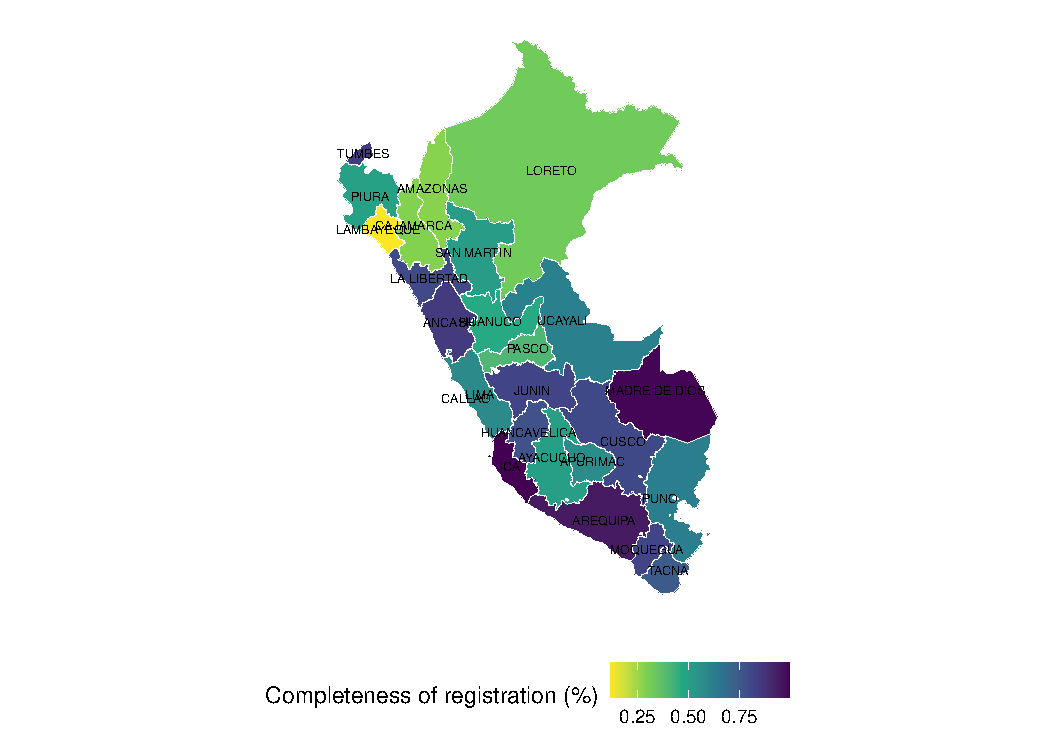
\includegraphics{article_files/figure-latex/map-1.pdf}
\caption{\label{fig:map}Completeness of registration}
\end{figure}

\hypertarget{figure-5}{%
\subsection{Figure 5}\label{figure-5}}

\begin{figure}
\centering
\includegraphics{article_files/figure-latex/growth-1.pdf}
\caption{\label{fig:growth}Estimated registration growth rate by age-groups}
\end{figure}

\hypertarget{figure-6}{%
\subsection{Figure 6}\label{figure-6}}

\begin{figure}
\centering
\includegraphics{article_files/figure-latex/predicted-1.pdf}
\caption{\label{fig:predicted}Predicted excess registered mortality}
\end{figure}

\hypertarget{figure-7}{%
\subsection{Figure 7}\label{figure-7}}

\begin{figure}
\centering
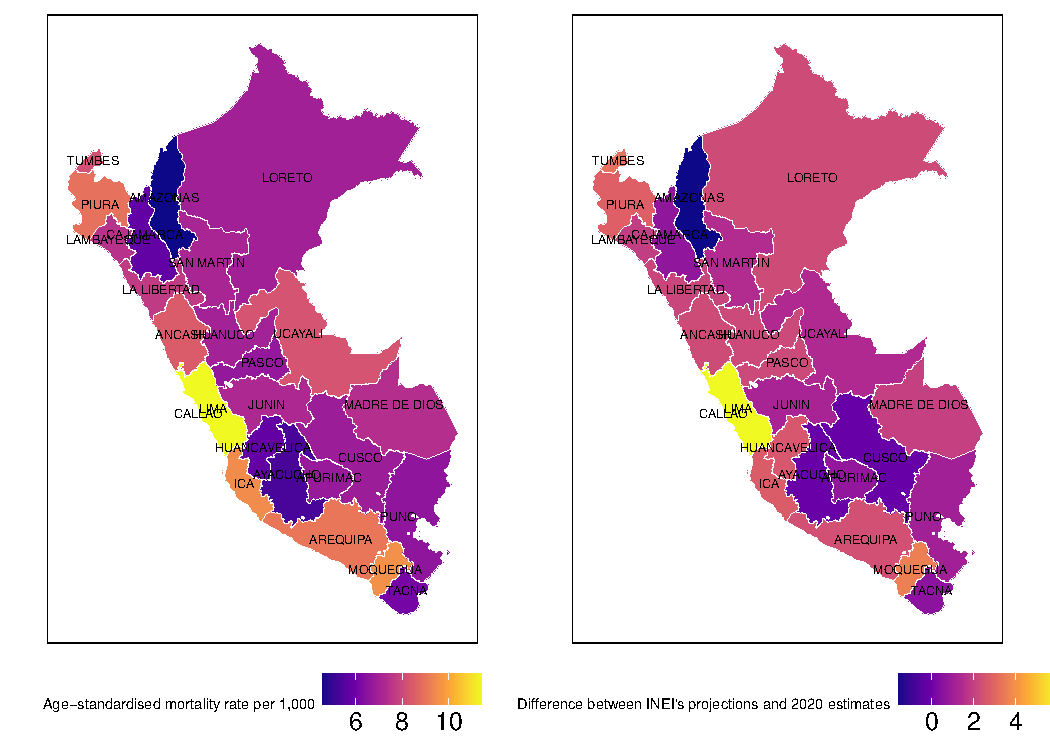
\includegraphics{article_files/figure-latex/map2-1.pdf}
\caption{\label{fig:map2}Age-standardised mortality rates}
\end{figure}

\hypertarget{table-1}{%
\subsection{Table 1}\label{table-1}}

\begin{longtable}[]{@{}cc@{}}
\caption{\label{tab:summary} Summary of estimations, Peru, 2020.}\tabularnewline
\toprule
Terms & Estimates (95\% CI) \\
\midrule
\endfirsthead
\toprule
Terms & Estimates (95\% CI) \\
\midrule
\endhead
Excess registered deaths & 94373 ( 79139 - 105767 ) \\
Completeness of CRVS deaths registration & 19.7 \% ( 24.3 \% - 30.6 \%) \\
Excess TOTAL mortality & 117574 ( 114101 - 139810 ) \\
Counterfactual estimated deaths in 2020 & 117276 ( 105882 - 132510 ) \\
Total estimated deaths in 2020 & 278499 ( 258902 - 322458 ) \\
\bottomrule
\end{longtable}

\hypertarget{table-2}{%
\subsection{Table 2}\label{table-2}}

\begin{longtable}[]{@{}
  >{\centering\arraybackslash}p{(\columnwidth - 14\tabcolsep) * \real{0.10}}
  >{\centering\arraybackslash}p{(\columnwidth - 14\tabcolsep) * \real{0.12}}
  >{\centering\arraybackslash}p{(\columnwidth - 14\tabcolsep) * \real{0.12}}
  >{\centering\arraybackslash}p{(\columnwidth - 14\tabcolsep) * \real{0.12}}
  >{\centering\arraybackslash}p{(\columnwidth - 14\tabcolsep) * \real{0.16}}
  >{\centering\arraybackslash}p{(\columnwidth - 14\tabcolsep) * \real{0.12}}
  >{\centering\arraybackslash}p{(\columnwidth - 14\tabcolsep) * \real{0.12}}
  >{\centering\arraybackslash}p{(\columnwidth - 14\tabcolsep) * \real{0.12}}@{}}
\caption{\label{tab:exineidepq}Estimated total excess deaths by region}\tabularnewline
\toprule
Region & Total excess (TE) & TE - Lower 95\% CI & TE - Upper 95\% CI & Excess registered (ER) & ER - Lower 95\% CI & ER - Upper 95\% CI & Excess Covid-19 \\
\midrule
\endfirsthead
\toprule
Region & Total excess (TE) & TE - Lower 95\% CI & TE - Upper 95\% CI & Excess registered (ER) & ER - Lower 95\% CI & ER - Upper 95\% CI & Excess Covid-19 \\
\midrule
\endhead
AMAZONAS & 179 & 179 & 179 & 0 & 0 & 0 & 179 \\
ANCASH & 3524 & 3241 & 4545 & 3470 & 2829 & 3980 & 54 \\
APURIMAC & 109 & 134 & 109 & 62.05 & 0.3284 & 99.3 & 109 \\
AREQUIPA & 5338 & 4812 & 6199 & 5322 & 4564 & 5912 & 16 \\
AYACUCHO & 422.5 & 333 & 794 & 355 & 132.2 & 520.1 & 67 \\
CAJAMARCA & 2151 & 2151 & 3253 & 1614 & 1113 & 1974 & 147 \\
CALLAO & 6759 & 6722 & 7830 & 6174 & 5643 & 6574 & 18 \\
CUSCO & 1800 & 1486 & 2624 & 1767 & 1225 & 2189 & 33 \\
HUANCAVELICA & 201.7 & 131.7 & 297.8 & 33.44 & -121.2 & 138.2 & 168 \\
HUANUCO & 963.1 & 596.9 & 1938 & 935.1 & 450.7 & 1289 & 28 \\
ICA & 4149 & 3637 & 4553 & 4081 & 3560 & 4474 & 68 \\
JUNIN & 2524 & 2120 & 3567 & 2498 & 1796 & 3040 & 26 \\
LA LIBERTAD & 6766 & 6690 & 8193 & 6452 & 5709 & 7026 & 5 \\
LAMBAYEQUE & 2096 & 1872 & 2827 & -2535 & -4967 & -909.5 & 4631 \\
LIMA & 61986 & 61918 & 69672 & 50932 & 47745 & 53674 & 83 \\
LORETO & 2607 & 2442 & 3496 & 1664 & 922 & 2152 & 451 \\
MADRE DE DIOS & 0 & 0 & 0 & 0 & 0 & 0 & 0 \\
MOQUEGUA & 363 & 320.6 & 453.1 & -147.8 & -441.1 & 52.94 & 511 \\
PASCO & 53 & 53 & 53 & 0 & 0 & 0 & 53 \\
PIURA & 8832 & 8727 & 10075 & 7320 & 6737 & 7754 & 35 \\
PUNO & 2787 & 2744 & 3802 & 2476 & 2030 & 2812 & 16 \\
SAN MARTIN & 2061 & 2010 & 2921 & 1558 & 967.9 & 1957 & 254 \\
TACNA & 368.5 & 309.4 & 536.4 & 250.5 & 146.4 & 321 & 118 \\
TUMBES & 450.4 & 388.7 & 537.6 & -343.7 & -866.3 & -0.5774 & 794 \\
UCAYALI & 1084 & 1084 & 1357 & 436.1 & -35.47 & 739.7 & 556 \\
Total & 117574 & 114101 & 139810 & 94373 & 79139 & 105767 & 8420 \\
\bottomrule
\end{longtable}

\hypertarget{table-3}{%
\subsection{Table 3}\label{table-3}}

\begin{longtable}[]{@{}
  >{\centering\arraybackslash}p{(\columnwidth - 14\tabcolsep) * \real{0.08}}
  >{\centering\arraybackslash}p{(\columnwidth - 14\tabcolsep) * \real{0.13}}
  >{\centering\arraybackslash}p{(\columnwidth - 14\tabcolsep) * \real{0.13}}
  >{\centering\arraybackslash}p{(\columnwidth - 14\tabcolsep) * \real{0.13}}
  >{\centering\arraybackslash}p{(\columnwidth - 14\tabcolsep) * \real{0.16}}
  >{\centering\arraybackslash}p{(\columnwidth - 14\tabcolsep) * \real{0.13}}
  >{\centering\arraybackslash}p{(\columnwidth - 14\tabcolsep) * \real{0.13}}
  >{\centering\arraybackslash}p{(\columnwidth - 14\tabcolsep) * \real{0.13}}@{}}
\caption{\label{tab:exineiageq} Estimated total excess deaths by age-group}\tabularnewline
\toprule
Age range & Total excess (TE) & TE - Lower 95\% CI & TE - Upper 95\% CI & Excess registered (ER) & ER - Lower 95\% CI & ER - Upper 95\% CI & Excess Covid-19 \\
\midrule
\endfirsthead
\toprule
Age range & Total excess (TE) & TE - Lower 95\% CI & TE - Upper 95\% CI & Excess registered (ER) & ER - Lower 95\% CI & ER - Upper 95\% CI & Excess Covid-19 \\
\midrule
\endhead
\textless{} 9 & 128 & 128.4 & 128.4 & -131.7 & -345.8 & -2.199 & 260 \\
10-19 & 46 & 46 & 46 & 28.1 & 10.56 & 38.56 & 46 \\
20-29 & 647 & 530.8 & 1071 & 483 & 250.6 & 654.6 & 164 \\
30-39 & 2352 & 2094 & 3251 & 1594 & 762.7 & 2162 & 591 \\
40-49 & 8021 & 7620 & 9533 & 6136 & 4617 & 7148 & 879 \\
50-59 & 17707 & 17360 & 20365 & 13624 & 11530 & 15094 & 1565 \\
60-69 & 28776 & 28292 & 32619 & 22401 & 19154 & 24752 & 2885 \\
70-79 & 29888 & 29320 & 34582 & 23925 & 20718 & 26399 & 1881 \\
\textgreater{} 80 & 30009 & 28710 & 38214 & 26314 & 22441 & 29521 & 150 \\
Total & 117574 & 114101 & 139810 & 94373 & 79139 & 105767 & 8421 \\
\bottomrule
\end{longtable}

\hypertarget{appendices}{%
\section{Appendices}\label{appendices}}

\hypertarget{appendix-1-model-fit-registration-completeness}{%
\subsection{Appendix 1: Model fit registration completeness}\label{appendix-1-model-fit-registration-completeness}}

\begin{longtable}[]{@{}
  >{\centering\arraybackslash}p{(\columnwidth - 6\tabcolsep) * \real{0.12}}
  >{\centering\arraybackslash}p{(\columnwidth - 6\tabcolsep) * \real{0.12}}
  >{\centering\arraybackslash}p{(\columnwidth - 6\tabcolsep) * \real{0.25}}
  >{\centering\arraybackslash}p{(\columnwidth - 6\tabcolsep) * \real{0.12}}@{}}
\caption{\label{tab:log} Model fit Mixed-effect logistic regression}\tabularnewline
\toprule
R2m & R2c & RMSE.normalised & RMSE \\
\midrule
\endfirsthead
\toprule
R2m & R2c & RMSE.normalised & RMSE \\
\midrule
\endhead
0.7438 & 0.8694 & 0.05282 & 0.2403 \\
\bottomrule
\end{longtable}

\hypertarget{quasi-poisson-models}{%
\subsubsection{Quasi-Poisson models}\label{quasi-poisson-models}}

\begin{longtable}[]{@{}
  >{\centering\arraybackslash}p{(\columnwidth - 26\tabcolsep) * \real{0.11}}
  >{\centering\arraybackslash}p{(\columnwidth - 26\tabcolsep) * \real{0.06}}
  >{\centering\arraybackslash}p{(\columnwidth - 26\tabcolsep) * \real{0.11}}
  >{\centering\arraybackslash}p{(\columnwidth - 26\tabcolsep) * \real{0.07}}
  >{\centering\arraybackslash}p{(\columnwidth - 26\tabcolsep) * \real{0.06}}
  >{\centering\arraybackslash}p{(\columnwidth - 26\tabcolsep) * \real{0.04}}
  >{\centering\arraybackslash}p{(\columnwidth - 26\tabcolsep) * \real{0.04}}
  >{\centering\arraybackslash}p{(\columnwidth - 26\tabcolsep) * \real{0.08}}
  >{\centering\arraybackslash}p{(\columnwidth - 26\tabcolsep) * \real{0.10}}
  >{\centering\arraybackslash}p{(\columnwidth - 26\tabcolsep) * \real{0.05}}
  >{\centering\arraybackslash}p{(\columnwidth - 26\tabcolsep) * \real{0.07}}
  >{\centering\arraybackslash}p{(\columnwidth - 26\tabcolsep) * \real{0.07}}
  >{\centering\arraybackslash}p{(\columnwidth - 26\tabcolsep) * \real{0.04}}
  >{\centering\arraybackslash}p{(\columnwidth - 26\tabcolsep) * \real{0.09}}@{}}
\caption{\label{tab:qpoisson} Model fit Quasi-Poisson}\tabularnewline
\toprule
Departamento & range & null.deviance & df.null & logLik & AIC & BIC & deviance & df.residual & nobs & fit & dif.dev & df & p \\
\midrule
\endfirsthead
\toprule
Departamento & range & null.deviance & df.null & logLik & AIC & BIC & deviance & df.residual & nobs & fit & dif.dev & df & p \\
\midrule
\endhead
AMAZONAS & a0.9 & 62.27 & 135 & NA & NA & NA & 52.23 & 119 & 136 & 0.1612 & 10.03 & 16 & 0.8648 \\
AMAZONAS & a10.19 & 23.19 & 76 & NA & NA & NA & 18.3 & 60 & 77 & 0.2112 & 4.898 & 16 & 0.9962 \\
AMAZONAS & a20.29 & 26.94 & 109 & NA & NA & NA & 20.89 & 93 & 110 & 0.2245 & 6.046 & 16 & 0.9876 \\
AMAZONAS & a30.39 & 42.37 & 122 & NA & NA & NA & 30.92 & 106 & 123 & 0.2703 & 11.45 & 16 & 0.7806 \\
AMAZONAS & a40.49 & 73.94 & 154 & NA & NA & NA & 65.59 & 138 & 155 & 0.1131 & 8.359 & 16 & 0.9374 \\
AMAZONAS & a50.59 & 135.5 & 173 & NA & NA & NA & 110.4 & 157 & 174 & 0.1855 & 25.15 & 16 & 0.06728 \\
AMAZONAS & a60.69 & 266.4 & 181 & NA & NA & NA & 166.3 & 164 & 182 & 0.3757 & 100.1 & 17 & 8.531e-14 \\
AMAZONAS & a70.79 & 229.6 & 198 & NA & NA & NA & 206.2 & 181 & 199 & 0.102 & 23.43 & 17 & 0.1359 \\
AMAZONAS & a80 & 256.4 & 203 & NA & NA & NA & 210.3 & 186 & 204 & 0.1796 & 46.04 & 17 & 0.0001702 \\
ANCASH & a0.9 & 220.7 & 204 & NA & NA & NA & 187.9 & 187 & 205 & 0.1487 & 32.81 & 17 & 0.0119 \\
ANCASH & a10.19 & 101.8 & 176 & NA & NA & NA & 93.9 & 159 & 177 & 0.07762 & 7.902 & 17 & 0.9686 \\
ANCASH & a20.29 & 159.5 & 196 & NA & NA & NA & 141.5 & 179 & 197 & 0.1128 & 18 & 17 & 0.3891 \\
ANCASH & a30.39 & 191.9 & 200 & NA & NA & NA & 159 & 183 & 201 & 0.1716 & 32.93 & 17 & 0.01151 \\
ANCASH & a40.49 & 357.4 & 205 & NA & NA & NA & 216.4 & 188 & 206 & 0.3946 & 141 & 17 & 1.393e-21 \\
ANCASH & a50.59 & 767.2 & 206 & NA & NA & NA & 243.7 & 189 & 207 & 0.6824 & 523.5 & 17 & 2.107e-100 \\
ANCASH & a60.69 & 1100 & 206 & NA & NA & NA & 248.5 & 189 & 207 & 0.774 & 851.1 & 17 & 5.733e-170 \\
ANCASH & a70.79 & 1088 & 206 & NA & NA & NA & 267.9 & 189 & 207 & 0.7537 & 819.8 & 17 & 2.723e-163 \\
ANCASH & a80 & 748.4 & 206 & NA & NA & NA & 250.5 & 189 & 207 & 0.6653 & 497.9 & 17 & 5.227e-95 \\
APURIMAC & a0.9 & 102.6 & 170 & NA & NA & NA & 90.44 & 154 & 171 & 0.1184 & 12.15 & 16 & 0.7339 \\
APURIMAC & a10.19 & 20.66 & 99 & NA & NA & NA & 16.27 & 83 & 100 & 0.2124 & 4.389 & 16 & 0.9981 \\
APURIMAC & a20.29 & 50.37 & 128 & NA & NA & NA & 40.86 & 112 & 129 & 0.1887 & 9.505 & 16 & 0.8912 \\
APURIMAC & a30.39 & 76.68 & 148 & NA & NA & NA & 67.06 & 132 & 149 & 0.1255 & 9.623 & 16 & 0.8856 \\
APURIMAC & a40.49 & 114.6 & 164 & NA & NA & NA & 104.8 & 148 & 165 & 0.08579 & 9.832 & 16 & 0.8752 \\
APURIMAC & a50.59 & 185.8 & 190 & NA & NA & NA & 142.9 & 173 & 191 & 0.2311 & 42.93 & 17 & 0.0004916 \\
APURIMAC & a60.69 & 292 & 199 & NA & NA & NA & 221.3 & 182 & 200 & 0.2424 & 70.79 & 17 & 1.578e-08 \\
APURIMAC & a70.79 & 263.7 & 206 & NA & NA & NA & 196 & 189 & 207 & 0.2568 & 67.73 & 17 & 5.28e-08 \\
APURIMAC & a80 & 372.9 & 206 & NA & NA & NA & 212.2 & 189 & 207 & 0.4311 & 160.7 & 17 & 1.901e-25 \\
AREQUIPA & a0.9 & 242.8 & 202 & NA & NA & NA & 213.4 & 185 & 203 & 0.1211 & 29.41 & 17 & 0.03095 \\
AREQUIPA & a10.19 & 106.2 & 167 & NA & NA & NA & 99.85 & 151 & 168 & 0.05988 & 6.36 & 16 & 0.9837 \\
AREQUIPA & a20.29 & 171.4 & 199 & NA & NA & NA & 153.1 & 182 & 200 & 0.107 & 18.33 & 17 & 0.3681 \\
AREQUIPA & a30.39 & 236.7 & 202 & NA & NA & NA & 186.4 & 185 & 203 & 0.2127 & 50.34 & 17 & 0.00003744 \\
AREQUIPA & a40.49 & 599.7 & 204 & NA & NA & NA & 250.6 & 187 & 205 & 0.5822 & 349.1 & 17 & 7.466e-64 \\
AREQUIPA & a50.59 & 1486 & 206 & NA & NA & NA & 325.6 & 189 & 207 & 0.7809 & 1160 & 17 & 4.311e-236 \\
AREQUIPA & a60.69 & 2417 & 206 & NA & NA & NA & 344.6 & 189 & 207 & 0.8574 & 2072 & 17 & 0 \\
AREQUIPA & a70.79 & 2435 & 206 & NA & NA & NA & 333.7 & 189 & 207 & 0.8629 & 2101 & 17 & 0 \\
AREQUIPA & a80 & 2587 & 206 & NA & NA & NA & 320.1 & 189 & 207 & 0.8763 & 2267 & 17 & 0 \\
AYACUCHO & a0.9 & 165.6 & 170 & NA & NA & NA & 123 & 154 & 171 & 0.2574 & 42.62 & 16 & 0.0003185 \\
AYACUCHO & a10.19 & 55.2 & 124 & NA & NA & NA & 49.19 & 108 & 125 & 0.1089 & 6.013 & 16 & 0.988 \\
AYACUCHO & a20.29 & 103.6 & 170 & NA & NA & NA & 85.56 & 154 & 171 & 0.1742 & 18.04 & 16 & 0.3214 \\
AYACUCHO & a30.39 & 92.51 & 159 & NA & NA & NA & 81.2 & 143 & 160 & 0.1222 & 11.3 & 16 & 0.7903 \\
AYACUCHO & a40.49 & 153.3 & 171 & NA & NA & NA & 121.8 & 155 & 172 & 0.2056 & 31.52 & 16 & 0.01155 \\
AYACUCHO & a50.59 & 212.8 & 190 & NA & NA & NA & 154.6 & 173 & 191 & 0.2734 & 58.18 & 17 & 2.09e-06 \\
AYACUCHO & a60.69 & 316.1 & 200 & NA & NA & NA & 175.2 & 183 & 201 & 0.4459 & 140.9 & 17 & 1.434e-21 \\
AYACUCHO & a70.79 & 443.8 & 203 & NA & NA & NA & 216 & 186 & 204 & 0.5134 & 227.9 & 17 & 6.674e-39 \\
AYACUCHO & a80 & 431.4 & 205 & NA & NA & NA & 190.6 & 188 & 206 & 0.5582 & 240.8 & 17 & 1.573e-41 \\
CAJAMARCA & a0.9 & 264.3 & 204 & NA & NA & NA & 228 & 187 & 205 & 0.1371 & 36.24 & 17 & 0.004261 \\
CAJAMARCA & a10.19 & 58.14 & 141 & NA & NA & NA & 52.72 & 125 & 142 & 0.09312 & 5.414 & 16 & 0.9933 \\
CAJAMARCA & a20.29 & 118.3 & 178 & NA & NA & NA & 99.37 & 161 & 179 & 0.1597 & 18.88 & 17 & 0.3354 \\
CAJAMARCA & a30.39 & 199.4 & 192 & NA & NA & NA & 153.6 & 175 & 193 & 0.2298 & 45.81 & 17 & 0.0001843 \\
CAJAMARCA & a40.49 & 221 & 200 & NA & NA & NA & 156.4 & 183 & 201 & 0.2924 & 64.61 & 17 & 1.791e-07 \\
CAJAMARCA & a50.59 & 532.6 & 205 & NA & NA & NA & 238.1 & 188 & 206 & 0.5529 & 294.5 & 17 & 1.532e-52 \\
CAJAMARCA & a60.69 & 865.8 & 206 & NA & NA & NA & 290.9 & 189 & 207 & 0.6641 & 575 & 17 & 2.825e-111 \\
CAJAMARCA & a70.79 & 691.9 & 206 & NA & NA & NA & 268.3 & 189 & 207 & 0.6123 & 423.7 & 17 & 2.076e-79 \\
CAJAMARCA & a80 & 531.5 & 206 & NA & NA & NA & 237.8 & 189 & 207 & 0.5527 & 293.7 & 17 & 2.205e-52 \\
CALLAO & a0.9 & 225.1 & 194 & NA & NA & NA & 211.3 & 177 & 195 & 0.06115 & 13.76 & 17 & 0.6838 \\
CALLAO & a10.19 & 56.25 & 133 & NA & NA & NA & 50.19 & 117 & 134 & 0.1076 & 6.054 & 16 & 0.9875 \\
CALLAO & a20.29 & 191.4 & 194 & NA & NA & NA & 174.2 & 177 & 195 & 0.08968 & 17.16 & 17 & 0.4433 \\
CALLAO & a30.39 & 252.6 & 201 & NA & NA & NA & 173.4 & 184 & 202 & 0.3134 & 79.17 & 17 & 5.381e-10 \\
CALLAO & a40.49 & 713.4 & 205 & NA & NA & NA & 226.5 & 188 & 206 & 0.6825 & 486.9 & 17 & 1.109e-92 \\
CALLAO & a50.59 & 1458 & 206 & NA & NA & NA & 303.8 & 189 & 207 & 0.7915 & 1154 & 17 & 1.119e-234 \\
CALLAO & a60.69 & 2350 & 206 & NA & NA & NA & 354.5 & 189 & 207 & 0.8492 & 1996 & 17 & 0 \\
CALLAO & a70.79 & 1970 & 206 & NA & NA & NA & 321.9 & 189 & 207 & 0.8366 & 1648 & 17 & 0 \\
CALLAO & a80 & 1412 & 206 & NA & NA & NA & 347.7 & 189 & 207 & 0.7538 & 1065 & 17 & 1.253e-215 \\
CUSCO & a0.9 & 284.1 & 206 & NA & NA & NA & 203.8 & 189 & 207 & 0.2828 & 80.35 & 17 & 3.321e-10 \\
CUSCO & a10.19 & 162.2 & 198 & NA & NA & NA & 136.9 & 181 & 199 & 0.1561 & 25.32 & 17 & 0.0878 \\
CUSCO & a20.29 & 247.8 & 203 & NA & NA & NA & 207.2 & 186 & 204 & 0.1637 & 40.55 & 17 & 0.001083 \\
CUSCO & a30.39 & 194.3 & 203 & NA & NA & NA & 150 & 186 & 204 & 0.2281 & 44.32 & 17 & 0.0003071 \\
CUSCO & a40.49 & 369 & 206 & NA & NA & NA & 265.8 & 189 & 207 & 0.2797 & 103.2 & 17 & 2.267e-14 \\
CUSCO & a50.59 & 456.4 & 206 & NA & NA & NA & 265.8 & 189 & 207 & 0.4175 & 190.6 & 17 & 2.246e-31 \\
CUSCO & a60.69 & 813.6 & 206 & NA & NA & NA & 326.6 & 189 & 207 & 0.5985 & 486.9 & 17 & 1.061e-92 \\
CUSCO & a70.79 & 663 & 206 & NA & NA & NA & 275.3 & 189 & 207 & 0.5848 & 387.7 & 17 & 6.791e-72 \\
CUSCO & a80 & 829.8 & 206 & NA & NA & NA & 280.9 & 189 & 207 & 0.6615 & 548.9 & 17 & 9.052e-106 \\
HUANCAVELICA & a0.9 & 174.5 & 197 & NA & NA & NA & 158.9 & 180 & 198 & 0.08932 & 15.58 & 17 & 0.5536 \\
HUANCAVELICA & a10.19 & 69.99 & 128 & NA & NA & NA & 54.2 & 112 & 129 & 0.2256 & 15.79 & 16 & 0.4679 \\
HUANCAVELICA & a20.29 & 73.45 & 146 & NA & NA & NA & 62.38 & 130 & 147 & 0.1508 & 11.07 & 16 & 0.8049 \\
HUANCAVELICA & a30.39 & 85.91 & 164 & NA & NA & NA & 77.44 & 148 & 165 & 0.09855 & 8.466 & 16 & 0.9338 \\
HUANCAVELICA & a40.49 & 162.6 & 177 & NA & NA & NA & 123.6 & 161 & 178 & 0.2396 & 38.96 & 16 & 0.001104 \\
HUANCAVELICA & a50.59 & 199.9 & 195 & NA & NA & NA & 158.2 & 178 & 196 & 0.2083 & 41.62 & 17 & 0.0007602 \\
HUANCAVELICA & a60.69 & 294.9 & 204 & NA & NA & NA & 232.9 & 187 & 205 & 0.2101 & 61.96 & 17 & 4.973e-07 \\
HUANCAVELICA & a70.79 & 352.3 & 205 & NA & NA & NA & 245.4 & 188 & 206 & 0.3035 & 106.9 & 17 & 4.561e-15 \\
HUANCAVELICA & a80 & 260.7 & 206 & NA & NA & NA & 198.9 & 189 & 207 & 0.2372 & 61.85 & 17 & 5.194e-07 \\
HUANUCO & a0.9 & 195.8 & 204 & NA & NA & NA & 176.3 & 187 & 205 & 0.09944 & 19.47 & 17 & 0.3023 \\
HUANUCO & a10.19 & 93.14 & 155 & NA & NA & NA & 82.54 & 139 & 156 & 0.1138 & 10.6 & 16 & 0.8335 \\
HUANUCO & a20.29 & 132 & 193 & NA & NA & NA & 113.8 & 176 & 194 & 0.138 & 18.22 & 17 & 0.3751 \\
HUANUCO & a30.39 & 156.4 & 191 & NA & NA & NA & 138.1 & 174 & 192 & 0.1174 & 18.37 & 17 & 0.3657 \\
HUANUCO & a40.49 & 227.2 & 200 & NA & NA & NA & 185.3 & 183 & 201 & 0.1844 & 41.9 & 17 & 0.0006929 \\
HUANUCO & a50.59 & 329.1 & 206 & NA & NA & NA & 251.4 & 189 & 207 & 0.2359 & 77.62 & 17 & 1.01e-09 \\
HUANUCO & a60.69 & 421.4 & 206 & NA & NA & NA & 216.3 & 189 & 207 & 0.4866 & 205.1 & 17 & 2.718e-34 \\
HUANUCO & a70.79 & 363.2 & 206 & NA & NA & NA & 218 & 189 & 207 & 0.3999 & 145.2 & 17 & 2.102e-22 \\
HUANUCO & a80 & 359.2 & 206 & NA & NA & NA & 225.1 & 189 & 207 & 0.3733 & 134.1 & 17 & 3.055e-20 \\
ICA & a0.9 & 157.3 & 200 & NA & NA & NA & 145 & 183 & 201 & 0.07817 & 12.29 & 17 & 0.7821 \\
ICA & a10.19 & 44.47 & 134 & NA & NA & NA & 42.52 & 118 & 135 & 0.0437 & 1.943 & 16 & 1 \\
ICA & a20.29 & 158.7 & 186 & NA & NA & NA & 137.8 & 169 & 187 & 0.1312 & 20.82 & 17 & 0.2344 \\
ICA & a30.39 & 236.1 & 195 & NA & NA & NA & 186.2 & 178 & 196 & 0.2114 & 49.91 & 17 & 0.00004362 \\
ICA & a40.49 & 556.1 & 205 & NA & NA & NA & 244.6 & 188 & 206 & 0.5601 & 311.5 & 17 & 4.692e-56 \\
ICA & a50.59 & 1030 & 206 & NA & NA & NA & 260.6 & 189 & 207 & 0.747 & 769.4 & 17 & 1.539e-152 \\
ICA & a60.69 & 1669 & 206 & NA & NA & NA & 307 & 189 & 207 & 0.816 & 1362 & 17 & 2.485e-279 \\
ICA & a70.79 & 1128 & 206 & NA & NA & NA & 288.1 & 189 & 207 & 0.7445 & 839.5 & 17 & 1.751e-167 \\
ICA & a80 & 932.6 & 206 & NA & NA & NA & 319.6 & 189 & 207 & 0.6573 & 613 & 17 & 2.527e-119 \\
JUNIN & a0.9 & 229.1 & 205 & NA & NA & NA & 212 & 188 & 206 & 0.07443 & 17.05 & 17 & 0.451 \\
JUNIN & a10.19 & 145.9 & 187 & NA & NA & NA & 130.6 & 170 & 188 & 0.1048 & 15.29 & 17 & 0.5748 \\
JUNIN & a20.29 & 198.7 & 205 & NA & NA & NA & 171.6 & 188 & 206 & 0.1361 & 27.05 & 17 & 0.05741 \\
JUNIN & a30.39 & 268.4 & 205 & NA & NA & NA & 211.4 & 188 & 206 & 0.2122 & 56.93 & 17 & 3.338e-06 \\
JUNIN & a40.49 & 426.1 & 205 & NA & NA & NA & 248.8 & 188 & 206 & 0.416 & 177.3 & 17 & 1.016e-28 \\
JUNIN & a50.59 & 814 & 206 & NA & NA & NA & 292.3 & 189 & 207 & 0.6409 & 521.7 & 17 & 5.092e-100 \\
JUNIN & a60.69 & 1019 & 206 & NA & NA & NA & 319.9 & 189 & 207 & 0.6859 & 698.7 & 17 & 1.655e-137 \\
JUNIN & a70.79 & 827.1 & 206 & NA & NA & NA & 259.1 & 189 & 207 & 0.6868 & 568.1 & 17 & 8.158e-110 \\
JUNIN & a80 & 730.8 & 206 & NA & NA & NA & 237.2 & 189 & 207 & 0.6755 & 493.7 & 17 & 4.042e-94 \\
LA LIBERTAD & a0.9 & 249.4 & 206 & NA & NA & NA & 229.9 & 189 & 207 & 0.078 & 19.45 & 17 & 0.3033 \\
LA LIBERTAD & a10.19 & 182.7 & 190 & NA & NA & NA & 154.9 & 173 & 191 & 0.1518 & 27.73 & 17 & 0.04814 \\
LA LIBERTAD & a20.29 & 251.2 & 204 & NA & NA & NA & 229.7 & 187 & 205 & 0.08543 & 21.46 & 17 & 0.2064 \\
LA LIBERTAD & a30.39 & 281.8 & 206 & NA & NA & NA & 219.3 & 189 & 207 & 0.2217 & 62.47 & 17 & 4.092e-07 \\
LA LIBERTAD & a40.49 & 524.4 & 206 & NA & NA & NA & 200.1 & 189 & 207 & 0.6184 & 324.3 & 17 & 1.088e-58 \\
LA LIBERTAD & a50.59 & 1406 & 206 & NA & NA & NA & 357.2 & 189 & 207 & 0.746 & 1049 & 17 & 3.037e-212 \\
LA LIBERTAD & a60.69 & 2229 & 206 & NA & NA & NA & 391.4 & 189 & 207 & 0.8244 & 1837 & 17 & 0 \\
LA LIBERTAD & a70.79 & 1934 & 206 & NA & NA & NA & 388.7 & 189 & 207 & 0.799 & 1546 & 17 & 7.565e-319 \\
LA LIBERTAD & a80 & 1272 & 206 & NA & NA & NA & 326.4 & 189 & 207 & 0.7433 & 945.3 & 17 & 4.386e-190 \\
LAMBAYEQUE & a0.9 & 340.7 & 181 & NA & NA & NA & 153.7 & 164 & 182 & 0.5489 & 187 & 17 & 1.137e-30 \\
LAMBAYEQUE & a10.19 & 57.98 & 118 & NA & NA & NA & 48.42 & 102 & 119 & 0.165 & 9.566 & 16 & 0.8883 \\
LAMBAYEQUE & a20.29 & 153.8 & 159 & NA & NA & NA & 105.9 & 143 & 160 & 0.3118 & 47.96 & 16 & 0.00004826 \\
LAMBAYEQUE & a30.39 & 207 & 173 & NA & NA & NA & 157.9 & 156 & 174 & 0.237 & 49.05 & 17 & 0.00005921 \\
LAMBAYEQUE & a40.49 & 581.6 & 182 & NA & NA & NA & 277.6 & 165 & 183 & 0.5227 & 304 & 17 & 1.7e-54 \\
LAMBAYEQUE & a50.59 & 1082 & 184 & NA & NA & NA & 320.7 & 167 & 185 & 0.7036 & 761.4 & 17 & 7.765e-151 \\
LAMBAYEQUE & a60.69 & 1985 & 193 & NA & NA & NA & 432.3 & 176 & 194 & 0.7823 & 1553 & 17 & 1.992e-320 \\
LAMBAYEQUE & a70.79 & 2114 & 199 & NA & NA & NA & 409.2 & 182 & 200 & 0.8065 & 1705 & 17 & 0 \\
LAMBAYEQUE & a80 & 3676 & 202 & NA & NA & NA & 654 & 185 & 203 & 0.8221 & 3022 & 17 & 0 \\
LIMA & a0.9 & 348.6 & 206 & NA & NA & NA & 268.7 & 189 & 207 & 0.2291 & 79.88 & 17 & 4.028e-10 \\
LIMA & a10.19 & 253.8 & 206 & NA & NA & NA & 213.1 & 189 & 207 & 0.1603 & 40.69 & 17 & 0.001034 \\
LIMA & a20.29 & 410.1 & 206 & NA & NA & NA & 286.5 & 189 & 207 & 0.3013 & 123.6 & 17 & 3.211e-18 \\
LIMA & a30.39 & 1254 & 206 & NA & NA & NA & 247.7 & 189 & 207 & 0.8025 & 1007 & 17 & 3.512e-203 \\
LIMA & a40.49 & 4855 & 206 & NA & NA & NA & 371.7 & 189 & 207 & 0.9234 & 4483 & 17 & 0 \\
LIMA & a50.59 & 12239 & 206 & NA & NA & NA & 726.3 & 189 & 207 & 0.9407 & 11512 & 17 & 0 \\
LIMA & a60.69 & 20219 & 206 & NA & NA & NA & 1021 & 189 & 207 & 0.9495 & 19198 & 17 & 0 \\
LIMA & a70.79 & 17310 & 206 & NA & NA & NA & 1008 & 189 & 207 & 0.9418 & 16301 & 17 & 0 \\
LIMA & a80 & 14400 & 206 & NA & NA & NA & 770 & 189 & 207 & 0.9465 & 13630 & 17 & 0 \\
LORETO & a0.9 & 225.3 & 204 & NA & NA & NA & 202 & 187 & 205 & 0.1036 & 23.35 & 17 & 0.1383 \\
LORETO & a10.19 & 84.68 & 150 & NA & NA & NA & 66.18 & 134 & 151 & 0.2185 & 18.5 & 16 & 0.2956 \\
LORETO & a20.29 & 148 & 190 & NA & NA & NA & 138.8 & 173 & 191 & 0.06196 & 9.169 & 17 & 0.9348 \\
LORETO & a30.39 & 234.6 & 199 & NA & NA & NA & 171 & 182 & 200 & 0.2709 & 63.54 & 17 & 2.705e-07 \\
LORETO & a40.49 & 412.2 & 202 & NA & NA & NA & 196.2 & 185 & 203 & 0.5239 & 216 & 17 & 1.732e-36 \\
LORETO & a50.59 & 806.8 & 204 & NA & NA & NA & 244.3 & 187 & 205 & 0.6971 & 562.4 & 17 & 1.261e-108 \\
LORETO & a60.69 & 1591 & 204 & NA & NA & NA & 404.9 & 187 & 205 & 0.7455 & 1186 & 17 & 1.105e-241 \\
LORETO & a70.79 & 1357 & 205 & NA & NA & NA & 310.5 & 188 & 206 & 0.7712 & 1047 & 17 & 9.906e-212 \\
LORETO & a80 & 806.5 & 206 & NA & NA & NA & 316.6 & 189 & 207 & 0.6074 & 489.8 & 17 & 2.626e-93 \\
MADRE DE DIOS & a0.9 & 78.23 & 130 & NA & NA & NA & 64.68 & 114 & 131 & 0.1733 & 13.55 & 16 & 0.6319 \\
MADRE DE DIOS & a10.19 & 16.24 & 78 & NA & NA & NA & 11.6 & 62 & 79 & 0.2857 & 4.64 & 16 & 0.9973 \\
MADRE DE DIOS & a20.29 & 75.72 & 151 & NA & NA & NA & 68.88 & 135 & 152 & 0.09032 & 6.839 & 16 & 0.9762 \\
MADRE DE DIOS & a30.39 & 72.37 & 139 & NA & NA & NA & 59.35 & 123 & 140 & 0.1799 & 13.02 & 16 & 0.6714 \\
MADRE DE DIOS & a40.49 & 99.54 & 149 & NA & NA & NA & 78.97 & 133 & 150 & 0.2066 & 20.57 & 16 & 0.1957 \\
MADRE DE DIOS & a50.59 & 205.3 & 162 & NA & NA & NA & 106.8 & 146 & 163 & 0.4795 & 98.44 & 16 & 6.796e-14 \\
MADRE DE DIOS & a60.69 & 251.4 & 170 & NA & NA & NA & 117.2 & 154 & 171 & 0.5337 & 134.2 & 16 & 9.861e-21 \\
MADRE DE DIOS & a70.79 & 197 & 168 & NA & NA & NA & 113.1 & 152 & 169 & 0.426 & 83.92 & 16 & 3.25e-11 \\
MADRE DE DIOS & a80 & 159.4 & 166 & NA & NA & NA & 103.2 & 150 & 167 & 0.3526 & 56.21 & 16 & 2.249e-06 \\
MOQUEGUA & a0.9 & 20.19 & 78 & NA & NA & NA & 16.97 & 62 & 79 & 0.1596 & 3.222 & 16 & 0.9997 \\
MOQUEGUA & a10.19 & 6.284 & 37 & NA & NA & NA & 2.998 & 21 & 38 & 0.523 & 3.287 & 16 & 0.9997 \\
MOQUEGUA & a20.29 & 16.63 & 82 & NA & NA & NA & 14.82 & 66 & 83 & 0.1088 & 1.809 & 16 & 1 \\
MOQUEGUA & a30.39 & 16.13 & 81 & NA & NA & NA & 13.5 & 65 & 82 & 0.1631 & 2.631 & 16 & 0.9999 \\
MOQUEGUA & a40.49 & 93.28 & 123 & NA & NA & NA & 50.43 & 107 & 124 & 0.4594 & 42.85 & 16 & 0.0002947 \\
MOQUEGUA & a50.59 & 242.7 & 151 & NA & NA & NA & 90.44 & 135 & 152 & 0.6274 & 152.3 & 16 & 2.762e-24 \\
MOQUEGUA & a60.69 & 550.9 & 184 & NA & NA & NA & 182.3 & 167 & 185 & 0.669 & 368.5 & 17 & 6.893e-68 \\
MOQUEGUA & a70.79 & 699.7 & 198 & NA & NA & NA & 230.7 & 181 & 199 & 0.6703 & 469 & 17 & 6.351e-89 \\
MOQUEGUA & a80 & 509.4 & 205 & NA & NA & NA & 224.4 & 188 & 206 & 0.5594 & 284.9 & 17 & 1.424e-50 \\
PASCO & a0.9 & 67.77 & 141 & NA & NA & NA & 50.3 & 125 & 142 & 0.2578 & 17.47 & 16 & 0.3558 \\
PASCO & a10.19 & 14.81 & 61 & NA & NA & NA & 9.727 & 45 & 62 & 0.3433 & 5.086 & 16 & 0.9953 \\
PASCO & a20.29 & 26.91 & 104 & NA & NA & NA & 25.35 & 88 & 105 & 0.05796 & 1.56 & 16 & 1 \\
PASCO & a30.39 & 51.29 & 106 & NA & NA & NA & 44.48 & 90 & 107 & 0.1327 & 6.805 & 16 & 0.9768 \\
PASCO & a40.49 & 61.74 & 130 & NA & NA & NA & 46.9 & 114 & 131 & 0.2403 & 14.84 & 16 & 0.5366 \\
PASCO & a50.59 & 138.8 & 156 & NA & NA & NA & 86.06 & 140 & 157 & 0.3799 & 52.72 & 16 & 8.365e-06 \\
PASCO & a60.69 & 192.3 & 166 & NA & NA & NA & 105 & 150 & 167 & 0.454 & 87.3 & 16 & 7.836e-12 \\
PASCO & a70.79 & 225.4 & 188 & NA & NA & NA & 150.2 & 171 & 189 & 0.3337 & 75.23 & 17 & 2.658e-09 \\
PASCO & a80 & 273.9 & 194 & NA & NA & NA & 202.1 & 177 & 195 & 0.262 & 71.74 & 17 & 1.079e-08 \\
PIURA & a0.9 & 246 & 206 & NA & NA & NA & 203.1 & 189 & 207 & 0.1742 & 42.87 & 17 & 0.0005021 \\
PIURA & a10.19 & 120.1 & 170 & NA & NA & NA & 106.5 & 154 & 171 & 0.1127 & 13.54 & 16 & 0.6333 \\
PIURA & a20.29 & 208.1 & 197 & NA & NA & NA & 165.8 & 180 & 198 & 0.203 & 42.24 & 17 & 0.0006183 \\
PIURA & a30.39 & 353 & 203 & NA & NA & NA & 210.1 & 186 & 204 & 0.4048 & 142.9 & 17 & 5.968e-22 \\
PIURA & a40.49 & 899.9 & 203 & NA & NA & NA & 319.1 & 186 & 204 & 0.6454 & 580.8 & 17 & 1.617e-112 \\
PIURA & a50.59 & 1575 & 206 & NA & NA & NA & 247.5 & 189 & 207 & 0.8428 & 1327 & 17 & 7.29e-272 \\
PIURA & a60.69 & 3123 & 206 & NA & NA & NA & 393.5 & 189 & 207 & 0.874 & 2729 & 17 & 0 \\
PIURA & a70.79 & 2392 & 206 & NA & NA & NA & 374.9 & 189 & 207 & 0.8433 & 2017 & 17 & 0 \\
PIURA & a80 & 1749 & 206 & NA & NA & NA & 385.8 & 189 & 207 & 0.7794 & 1363 & 17 & 1.32e-279 \\
PUNO & a0.9 & 225.3 & 205 & NA & NA & NA & 169.3 & 188 & 206 & 0.2486 & 56.01 & 17 & 4.713e-06 \\
PUNO & a10.19 & 126.6 & 180 & NA & NA & NA & 119.8 & 164 & 181 & 0.053 & 6.708 & 16 & 0.9785 \\
PUNO & a20.29 & 191.2 & 202 & NA & NA & NA & 179.7 & 185 & 203 & 0.0601 & 11.49 & 17 & 0.83 \\
PUNO & a30.39 & 295 & 206 & NA & NA & NA & 266.4 & 189 & 207 & 0.09692 & 28.59 & 17 & 0.03852 \\
PUNO & a40.49 & 370.5 & 206 & NA & NA & NA & 220.7 & 189 & 207 & 0.4042 & 149.7 & 17 & 2.755e-23 \\
PUNO & a50.59 & 730.5 & 206 & NA & NA & NA & 297.9 & 189 & 207 & 0.5922 & 432.6 & 17 & 2.77e-81 \\
PUNO & a60.69 & 959.1 & 206 & NA & NA & NA & 274 & 189 & 207 & 0.7143 & 685.1 & 17 & 1.264e-134 \\
PUNO & a70.79 & 863.2 & 206 & NA & NA & NA & 283.6 & 189 & 207 & 0.6715 & 579.6 & 17 & 2.976e-112 \\
PUNO & a80 & 703.8 & 206 & NA & NA & NA & 264.2 & 189 & 207 & 0.6246 & 439.6 & 17 & 9.301e-83 \\
SAN MARTIN & a0.9 & 239.4 & 203 & NA & NA & NA & 189.5 & 186 & 204 & 0.2086 & 49.95 & 17 & 0.00004294 \\
SAN MARTIN & a10.19 & 95.83 & 149 & NA & NA & NA & 77.58 & 133 & 150 & 0.1905 & 18.25 & 16 & 0.3093 \\
SAN MARTIN & a20.29 & 125.7 & 191 & NA & NA & NA & 115.5 & 174 & 192 & 0.08163 & 10.26 & 17 & 0.8922 \\
SAN MARTIN & a30.39 & 204.8 & 198 & NA & NA & NA & 153.4 & 181 & 199 & 0.2508 & 51.35 & 17 & 0.00002602 \\
SAN MARTIN & a40.49 & 313.7 & 205 & NA & NA & NA & 195.7 & 188 & 206 & 0.376 & 118 & 17 & 3.783e-17 \\
SAN MARTIN & a50.59 & 487.4 & 204 & NA & NA & NA & 244 & 187 & 205 & 0.4994 & 243.4 & 17 & 4.6e-42 \\
SAN MARTIN & a60.69 & 763.5 & 206 & NA & NA & NA & 268.7 & 189 & 207 & 0.6481 & 494.8 & 17 & 2.406e-94 \\
SAN MARTIN & a70.79 & 566.7 & 205 & NA & NA & NA & 222.8 & 188 & 206 & 0.6068 & 343.9 & 17 & 9.189e-63 \\
SAN MARTIN & a80 & 743.5 & 206 & NA & NA & NA & 292.9 & 189 & 207 & 0.6061 & 450.6 & 17 & 4.633e-85 \\
TACNA & a0.9 & 54.54 & 124 & NA & NA & NA & 42.79 & 108 & 125 & 0.2154 & 11.75 & 16 & 0.7611 \\
TACNA & a10.19 & 6.653 & 61 & NA & NA & NA & 4.638 & 45 & 62 & 0.3028 & 2.015 & 16 & 1 \\
TACNA & a20.29 & 47.05 & 115 & NA & NA & NA & 41.87 & 99 & 116 & 0.1102 & 5.184 & 16 & 0.9948 \\
TACNA & a30.39 & 83.11 & 154 & NA & NA & NA & 77.19 & 138 & 155 & 0.07122 & 5.919 & 16 & 0.9889 \\
TACNA & a40.49 & 156.1 & 172 & NA & NA & NA & 111.8 & 156 & 173 & 0.2839 & 44.32 & 16 & 0.0001761 \\
TACNA & a50.59 & 329.6 & 186 & NA & NA & NA & 204 & 169 & 187 & 0.3812 & 125.7 & 17 & 1.279e-18 \\
TACNA & a60.69 & 610.7 & 201 & NA & NA & NA & 262.3 & 184 & 202 & 0.5705 & 348.4 & 17 & 1.057e-63 \\
TACNA & a70.79 & 464.9 & 204 & NA & NA & NA & 263.4 & 187 & 205 & 0.4333 & 201.4 & 17 & 1.466e-33 \\
TACNA & a80 & 358.3 & 206 & NA & NA & NA & 245.3 & 189 & 207 & 0.3152 & 112.9 & 17 & 3.375e-16 \\
TUMBES & a0.9 & 53.94 & 133 & NA & NA & NA & 46.03 & 117 & 134 & 0.1466 & 7.907 & 16 & 0.9516 \\
TUMBES & a10.19 & 5.624 & 57 & NA & NA & NA & 3.076 & 41 & 58 & 0.453 & 2.548 & 16 & 0.9999 \\
TUMBES & a20.29 & 26.32 & 107 & NA & NA & NA & 21.66 & 91 & 108 & 0.177 & 4.658 & 16 & 0.9972 \\
TUMBES & a30.39 & 52.44 & 136 & NA & NA & NA & 39.35 & 120 & 137 & 0.2496 & 13.09 & 16 & 0.666 \\
TUMBES & a40.49 & 93.67 & 152 & NA & NA & NA & 65.36 & 136 & 153 & 0.3023 & 28.31 & 16 & 0.02899 \\
TUMBES & a50.59 & 267.8 & 174 & NA & NA & NA & 136.6 & 157 & 175 & 0.4898 & 131.2 & 17 & 1.121e-19 \\
TUMBES & a60.69 & 491.9 & 195 & NA & NA & NA & 199.6 & 178 & 196 & 0.5942 & 292.3 & 17 & 4.389e-52 \\
TUMBES & a70.79 & 368.9 & 195 & NA & NA & NA & 181.5 & 178 & 196 & 0.5081 & 187.4 & 17 & 9.411e-31 \\
TUMBES & a80 & 384.6 & 205 & NA & NA & NA & 224.7 & 188 & 206 & 0.4158 & 159.9 & 17 & 2.795e-25 \\
UCAYALI & a0.9 & 199.1 & 192 & NA & NA & NA & 153.7 & 175 & 193 & 0.228 & 45.41 & 17 & 0.0002117 \\
UCAYALI & a10.19 & 45.36 & 123 & NA & NA & NA & 36.37 & 107 & 124 & 0.1982 & 8.99 & 16 & 0.9138 \\
UCAYALI & a20.29 & 167.7 & 176 & NA & NA & NA & 146.9 & 159 & 177 & 0.1241 & 20.82 & 17 & 0.2347 \\
UCAYALI & a30.39 & 173.3 & 176 & NA & NA & NA & 138.5 & 159 & 177 & 0.2007 & 34.79 & 17 & 0.006621 \\
UCAYALI & a40.49 & 242 & 198 & NA & NA & NA & 198 & 181 & 199 & 0.1819 & 44.02 & 17 & 0.00034 \\
UCAYALI & a50.59 & 483.2 & 200 & NA & NA & NA & 247.6 & 183 & 201 & 0.4875 & 235.6 & 17 & 1.84e-40 \\
UCAYALI & a60.69 & 701.2 & 206 & NA & NA & NA & 250.9 & 189 & 207 & 0.6422 & 450.4 & 17 & 5.224e-85 \\
UCAYALI & a70.79 & 915.9 & 203 & NA & NA & NA & 284.7 & 186 & 204 & 0.6891 & 631.2 & 17 & 3.515e-123 \\
UCAYALI & a80 & 613.5 & 205 & NA & NA & NA & 310.4 & 188 & 206 & 0.4941 & 303.2 & 17 & 2.518e-54 \\
\bottomrule
\end{longtable}

\hypertarget{under-registration-rates}{%
\subsubsection{Under-registration rates}\label{under-registration-rates}}

\begin{longtable}[]{@{}
  >{\centering\arraybackslash}p{(\columnwidth - 2\tabcolsep) * \real{0.22}}
  >{\centering\arraybackslash}p{(\columnwidth - 2\tabcolsep) * \real{0.15}}@{}}
\caption{\label{tab:under} Under-registration rates}\tabularnewline
\toprule
Departamento & sub.mean \\
\midrule
\endfirsthead
\toprule
Departamento & sub.mean \\
\midrule
\endhead
ICA & 99.85 \\
MADRE DE DIOS & 99.17 \\
AREQUIPA & 94.81 \\
ANCASH & 85.12 \\
TUMBES & 85.04 \\
JUNIN & 82.32 \\
MOQUEGUA & 82.15 \\
CUSCO & 80.81 \\
LA LIBERTAD & 80.42 \\
HUANCAVELICA & 77.77 \\
CALLAO & 77.49 \\
TACNA & 74.44 \\
PUNO & 62.28 \\
UCAYALI & 61.8 \\
LIMA & 58.01 \\
APURIMAC & 57 \\
SAN MARTIN & 51.53 \\
AYACUCHO & 50.53 \\
PIURA & 49.41 \\
HUANUCO & 46.54 \\
PASCO & 40.6 \\
LORETO & 32.09 \\
CAJAMARCA & 28.41 \\
AMAZONAS & 27.99 \\
LAMBAYEQUE & 11.89 \\
\bottomrule
\end{longtable}

\hypertarget{age-standardised-deaths-rates}{%
\subsubsection{Age-standardised deaths rates}\label{age-standardised-deaths-rates}}

\begin{longtable}[]{@{}
  >{\centering\arraybackslash}p{(\columnwidth - 14\tabcolsep) * \real{0.19}}
  >{\centering\arraybackslash}p{(\columnwidth - 14\tabcolsep) * \real{0.13}}
  >{\centering\arraybackslash}p{(\columnwidth - 14\tabcolsep) * \real{0.10}}
  >{\centering\arraybackslash}p{(\columnwidth - 14\tabcolsep) * \real{0.10}}
  >{\centering\arraybackslash}p{(\columnwidth - 14\tabcolsep) * \real{0.16}}
  >{\centering\arraybackslash}p{(\columnwidth - 14\tabcolsep) * \real{0.08}}
  >{\centering\arraybackslash}p{(\columnwidth - 14\tabcolsep) * \real{0.08}}
  >{\centering\arraybackslash}p{(\columnwidth - 14\tabcolsep) * \real{0.16}}@{}}
\caption{\label{tab:standard} Age-standardised deaths rates}\tabularnewline
\toprule
Departamento & adj.rate & lci & uci & crude.rate & 2010 & 2015 & Difference \\
\midrule
\endfirsthead
\toprule
Departamento & adj.rate & lci & uci & crude.rate & 2010 & 2015 & Difference \\
\midrule
\endhead
AMAZONAS & 4.925 & 4.716 & 5.14 & 4.929 & 6.05 & 6.19 & -1.261 \\
ANCASH & 7.973 & 7.813 & 8.136 & 7.949 & 6.09 & 6.15 & 1.799 \\
APURIMAC & 6.745 & 6.512 & 6.985 & 7.324 & 6.76 & 6.61 & 0.7143 \\
AREQUIPA & 8.737 & 8.58 & 8.895 & 7.924 & 5.53 & 5.8 & 2.124 \\
AYACUCHO & 5.046 & 4.884 & 5.212 & 5.479 & 6.15 & 5.91 & -0.4305 \\
CAJAMARCA & 5.255 & 5.141 & 5.37 & 5.582 & 5.39 & 5.5 & 0.08242 \\
CALLAO & 10.25 & 10.06 & 10.44 & 9.808 & 4.91 & 5.27 & 4.538 \\
CUSCO & 6.524 & 6.389 & 6.662 & 6.502 & 6.88 & 6.97 & -0.4678 \\
HUANCAVELICA & 6.103 & 5.891 & 6.321 & 8.551 & 5.83 & 5.54 & 3.011 \\
HUANUCO & 6.444 & 6.279 & 6.613 & 7.534 & 5.94 & 5.98 & 1.554 \\
ICA & 9.498 & 9.289 & 9.711 & 8.036 & 4.99 & 5.29 & 2.746 \\
JUNIN & 6.863 & 6.726 & 7.002 & 7.049 & 6.17 & 6.24 & 0.8089 \\
LA LIBERTAD & 7.165 & 7.048 & 7.284 & 7.011 & 5.24 & 5.39 & 1.621 \\
LAMBAYEQUE & 12.71 & 12.51 & 12.9 & 12.7 & 5.25 & 5.55 & 7.147 \\
LIMA & 10.45 & 10.39 & 10.51 & 10.43 & 5.13 & 5.4 & 5.03 \\
LORETO & 6.7 & 6.547 & 6.856 & 7.077 & 4.92 & 5.07 & 2.007 \\
MADRE DE DIOS & 7.096 & 6.681 & 7.531 & 6.253 & 4.4 & 4.54 & 1.713 \\
MOQUEGUA & 12.34 & 11.84 & 12.85 & 12.14 & 5.49 & 5.86 & 6.282 \\
PASCO & 6.323 & 6.048 & 6.607 & 7.318 & 5.54 & 5.54 & 1.778 \\
PIURA & 7.752 & 7.628 & 7.878 & 7.247 & 5.36 & 5.5 & 1.747 \\
PUNO & 6.086 & 5.962 & 6.213 & 7.302 & 7.01 & 6.86 & 0.4425 \\
SAN MARTIN & 6.705 & 6.536 & 6.877 & 6.667 & 5.47 & 5.63 & 1.037 \\
TACNA & 6.227 & 5.973 & 6.49 & 6.082 & 5.09 & 5.4 & 0.6821 \\
TUMBES & 11.49 & 11.08 & 11.92 & 11.48 & 4.7 & 4.94 & 6.543 \\
UCAYALI & 8.931 & 8.676 & 9.19 & 7.93 & 5.68 & 5.93 & 2 \\
\bottomrule
\end{longtable}

\hypertarget{counterfacutual-and-total-deaths-2020}{%
\subsubsection{Counterfacutual and total deaths 2020}\label{counterfacutual-and-total-deaths-2020}}

\begin{longtable}[]{@{}
  >{\centering\arraybackslash}p{(\columnwidth - 28\tabcolsep) * \real{0.09}}
  >{\centering\arraybackslash}p{(\columnwidth - 28\tabcolsep) * \real{0.05}}
  >{\centering\arraybackslash}p{(\columnwidth - 28\tabcolsep) * \real{0.06}}
  >{\centering\arraybackslash}p{(\columnwidth - 28\tabcolsep) * \real{0.07}}
  >{\centering\arraybackslash}p{(\columnwidth - 28\tabcolsep) * \real{0.07}}
  >{\centering\arraybackslash}p{(\columnwidth - 28\tabcolsep) * \real{0.07}}
  >{\centering\arraybackslash}p{(\columnwidth - 28\tabcolsep) * \real{0.08}}
  >{\centering\arraybackslash}p{(\columnwidth - 28\tabcolsep) * \real{0.09}}
  >{\centering\arraybackslash}p{(\columnwidth - 28\tabcolsep) * \real{0.09}}
  >{\centering\arraybackslash}p{(\columnwidth - 28\tabcolsep) * \real{0.05}}
  >{\centering\arraybackslash}p{(\columnwidth - 28\tabcolsep) * \real{0.06}}
  >{\centering\arraybackslash}p{(\columnwidth - 28\tabcolsep) * \real{0.06}}
  >{\centering\arraybackslash}p{(\columnwidth - 28\tabcolsep) * \real{0.05}}
  >{\centering\arraybackslash}p{(\columnwidth - 28\tabcolsep) * \real{0.06}}
  >{\centering\arraybackslash}p{(\columnwidth - 28\tabcolsep) * \real{0.06}}@{}}
\caption{\label{tab:count} Counterfacutual and total deaths 2020}\tabularnewline
\toprule
Departamento & range & sinadef & excess.T & excess.l & excess.u & excess.reg & excess.reg.l & excess.reg.u & count & count.l & count.u & total & total.l & total.u \\
\midrule
\endfirsthead
\toprule
Departamento & range & sinadef & excess.T & excess.l & excess.u & excess.reg & excess.reg.l & excess.reg.u & count & count.l & count.u & total & total.l & total.u \\
\midrule
\endhead
AMAZONAS & a0.9 & 60 & 0 & 0 & 0 & 0 & 0 & 0 & 60 & 60 & 60 & 103.2 & 103.2 & 103.2 \\
AMAZONAS & a10.19 & 22 & 0 & 0 & 0 & 0 & 0 & 0 & 22 & 22 & 22 & 37.84 & 37.84 & 37.84 \\
AMAZONAS & a20.29 & 36 & 0 & 0 & 0 & 0 & 0 & 0 & 36 & 36 & 36 & 61.92 & 61.92 & 61.92 \\
AMAZONAS & a30.39 & 60 & 0 & 0 & 0 & 0 & 0 & 0 & 60 & 60 & 60 & 103.2 & 103.2 & 103.2 \\
AMAZONAS & a40.49 & 83 & 0 & 0 & 0 & 0 & 0 & 0 & 83 & 83 & 83 & 142.8 & 142.8 & 142.8 \\
AMAZONAS & a50.59 & 123 & 0 & 0 & 0 & 0 & 0 & 0 & 123 & 123 & 123 & 211.6 & 211.6 & 211.6 \\
AMAZONAS & a60.69 & 199 & 61 & 61 & 61 & 0 & 0 & 0 & 199 & 199 & 199 & 403.3 & 403.3 & 403.3 \\
AMAZONAS & a70.79 & 199 & 62 & 62 & 62 & 0 & 0 & 0 & 199 & 199 & 199 & 404.3 & 404.3 & 404.3 \\
AMAZONAS & a80 & 337 & 56 & 56 & 56 & 0 & 0 & 0 & 337 & 337 & 337 & 635.7 & 635.7 & 635.7 \\
ANCASH & a0.9 & 243 & 3 & 3 & 3 & 0 & 0 & 0 & 243 & 243 & 243 & 282.2 & 282.2 & 282.2 \\
ANCASH & a10.19 & 101 & 2 & 2 & 2 & 0 & 0 & 0 & 101 & 101 & 101 & 118 & 118 & 118 \\
ANCASH & a20.29 & 163 & 12 & 12 & 12 & 0 & 0 & 0 & 163 & 163 & 163 & 199.3 & 199.3 & 199.3 \\
ANCASH & a30.39 & 224 & 37 & 37 & 37 & 0 & 0 & 0 & 224 & 224 & 224 & 294.3 & 294.3 & 294.3 \\
ANCASH & a40.49 & 471 & 250.6 & 221.2 & 329.6 & 250.6 & 193.8 & 289.1 & 220.4 & 181.9 & 277.2 & 503.8 & 430.1 & 648.2 \\
ANCASH & a50.59 & 890 & 572.4 & 554.3 & 700 & 572.4 & 496.3 & 626.9 & 317.6 & 263.1 & 393.7 & 937.3 & 856.6 & 1152 \\
ANCASH & a60.69 & 1390 & 873.8 & 866 & 1053 & 873.8 & 778.4 & 946.4 & 516.2 & 443.6 & 611.6 & 1467 & 1376 & 1755 \\
ANCASH & a70.79 & 1960 & 1041 & 1012 & 1304 & 1041 & 896.5 & 1155 & 919.5 & 804.5 & 1064 & 2097 & 1936 & 2526 \\
ANCASH & a80 & 3130 & 732.5 & 533.2 & 1105 & 732.5 & 464 & 961.9 & 2398 & 2168 & 2666 & 3487 & 3024 & 4167 \\
APURIMAC & a0.9 & 100 & 0 & 0 & 0 & 0 & 0 & 0 & 100 & 100 & 100 & 143 & 143 & 143 \\
APURIMAC & a10.19 & 51 & 0 & 0 & 0 & 0 & 0 & 0 & 51 & 51 & 51 & 72.93 & 72.93 & 72.93 \\
APURIMAC & a20.29 & 64 & 0 & 0 & 0 & 0 & 0 & 0 & 64 & 64 & 64 & 91.52 & 91.52 & 91.52 \\
APURIMAC & a30.39 & 73 & 0 & 0 & 0 & 0 & 0 & 0 & 73 & 73 & 73 & 104.4 & 104.4 & 104.4 \\
APURIMAC & a40.49 & 119 & 0 & 0 & 0 & 0 & 0 & 0 & 119 & 119 & 119 & 170.2 & 170.2 & 170.2 \\
APURIMAC & a50.59 & 200 & 26 & 26 & 26 & 0 & 0 & 0 & 200 & 200 & 200 & 312 & 312 & 312 \\
APURIMAC & a60.69 & 275 & 0 & 25 & 0 & 62.05 & 0.3284 & 99.3 & 212.9 & 175.7 & 274.7 & 304.5 & 276.2 & 392.8 \\
APURIMAC & a70.79 & 447 & 39 & 39 & 39 & 0 & 0 & 0 & 447 & 447 & 447 & 678.2 & 678.2 & 678.2 \\
APURIMAC & a80 & 863 & 44 & 44 & 44 & 0 & 0 & 0 & 863 & 863 & 863 & 1278 & 1278 & 1278 \\
AREQUIPA & a0.9 & 216 & 4 & 4 & 4 & 0 & 0 & 0 & 216 & 216 & 216 & 231.2 & 231.2 & 231.2 \\
AREQUIPA & a10.19 & 98 & 0 & 0 & 0 & 0 & 0 & 0 & 98 & 98 & 98 & 103.1 & 103.1 & 103.1 \\
AREQUIPA & a20.29 & 232 & 12 & 12 & 12 & 0 & 0 & 0 & 232 & 232 & 232 & 256 & 256 & 256 \\
AREQUIPA & a30.39 & 329 & 61.79 & 29 & 105.3 & 61.79 & 6.422 & 99.39 & 267.2 & 229.6 & 322.6 & 342.9 & 270.5 & 444.6 \\
AREQUIPA & a40.49 & 662 & 313.8 & 250.2 & 381 & 313.8 & 239.5 & 365.2 & 348.2 & 296.8 & 422.5 & 680.1 & 562.5 & 825.4 \\
AREQUIPA & a50.59 & 1213 & 725.6 & 664.7 & 831.4 & 725.6 & 632.9 & 792 & 487.4 & 421 & 580.1 & 1238 & 1108 & 1442 \\
AREQUIPA & a60.69 & 1990 & 1160 & 1063 & 1317 & 1160 & 1022 & 1266 & 829.7 & 724.1 & 968.5 & 2033 & 1824 & 2336 \\
AREQUIPA & a70.79 & 2480 & 1279 & 1164 & 1475 & 1279 & 1113 & 1411 & 1201 & 1069 & 1367 & 2542 & 2289 & 2912 \\
AREQUIPA & a80 & 4307 & 1782 & 1625 & 2073 & 1782 & 1551 & 1979 & 2525 & 2328 & 2756 & 4438 & 4074 & 4973 \\
AYACUCHO & a0.9 & 122 & 0 & 0 & 0 & 0 & 0 & 0 & 122 & 122 & 122 & 182.3 & 182.3 & 182.3 \\
AYACUCHO & a10.19 & 62 & 0 & 0 & 0 & 0 & 0 & 0 & 62 & 62 & 62 & 92.67 & 92.67 & 92.67 \\
AYACUCHO & a20.29 & 94 & 0 & 0 & 0 & 0 & 0 & 0 & 94 & 94 & 94 & 140.5 & 140.5 & 140.5 \\
AYACUCHO & a30.39 & 100 & 0 & 0 & 0 & 0 & 0 & 0 & 100 & 100 & 100 & 149.5 & 149.5 & 149.5 \\
AYACUCHO & a40.49 & 161 & 0 & 0 & 0 & 0 & 0 & 0 & 161 & 161 & 161 & 240.6 & 240.6 & 240.6 \\
AYACUCHO & a50.59 & 214 & 50 & 50 & 50 & 0 & 0 & 0 & 214 & 214 & 214 & 369.9 & 369.9 & 369.9 \\
AYACUCHO & a60.69 & 373 & 100 & 100 & 164.8 & 82.51 & 31.85 & 117.5 & 290.5 & 255.5 & 341.1 & 534.2 & 481.8 & 674.7 \\
AYACUCHO & a70.79 & 554 & 132.7 & 105 & 268.9 & 132.7 & 61.26 & 184.4 & 421.3 & 369.6 & 492.7 & 762.4 & 657.5 & 1005 \\
AYACUCHO & a80 & 842 & 139.8 & 78 & 310.2 & 139.8 & 39.08 & 218.2 & 702.2 & 623.8 & 802.9 & 1189 & 1010 & 1510 \\
CAJAMARCA & a0.9 & 231 & 2 & 2 & 2 & -68.2 & -179.8 & -0.1757 & 299.2 & 231.2 & 410.8 & 515.4 & 398.7 & 706.9 \\
CAJAMARCA & a10.19 & 75 & 0 & 0 & 0 & 0 & 0 & 0 & 75 & 75 & 75 & 128.7 & 128.7 & 128.7 \\
CAJAMARCA & a20.29 & 128 & 6 & 6 & 6 & 0 & 0 & 0 & 128 & 128 & 128 & 225.6 & 225.6 & 225.6 \\
CAJAMARCA & a30.39 & 207 & 24 & 24 & 24 & 0 & 0 & 0 & 207 & 207 & 207 & 379.2 & 379.2 & 379.2 \\
CAJAMARCA & a40.49 & 294 & 47 & 47 & 47 & 0 & 0 & 0 & 294 & 294 & 294 & 551.5 & 551.5 & 551.5 \\
CAJAMARCA & a50.59 & 538 & 304.5 & 304.5 & 470.3 & 265.1 & 199.5 & 308.3 & 272.9 & 229.7 & 338.5 & 772.7 & 698.5 & 1051 \\
CAJAMARCA & a60.69 & 792 & 659.1 & 659.1 & 832.8 & 487.4 & 421.4 & 532.5 & 304.6 & 259.5 & 370.6 & 1182 & 1104 & 1469 \\
CAJAMARCA & a70.79 & 1072 & 554 & 554 & 854.2 & 448.4 & 342.3 & 527.8 & 623.6 & 544.2 & 729.7 & 1624 & 1488 & 2106 \\
CAJAMARCA & a80 & 1753 & 554 & 554 & 1016 & 481.2 & 329.8 & 605.3 & 1272 & 1148 & 1423 & 2736 & 2523 & 3459 \\
CALLAO & a0.9 & 156 & 3 & 3 & 3 & 0 & 0 & 0 & 156 & 156 & 156 & 194.1 & 194.1 & 194.1 \\
CALLAO & a10.19 & 49 & 0 & 0 & 0 & 0 & 0 & 0 & 49 & 49 & 49 & 60.03 & 60.03 & 60.03 \\
CALLAO & a20.29 & 185 & 15 & 15 & 15 & 0 & 0 & 0 & 185 & 185 & 185 & 241.7 & 241.7 & 241.7 \\
CALLAO & a30.39 & 319 & 119.6 & 82.57 & 186.6 & 119.6 & 67.59 & 153.5 & 199.4 & 165.5 & 251.4 & 363.9 & 285.3 & 494.6 \\
CALLAO & a40.49 & 639 & 525.1 & 525.1 & 606.6 & 478.5 & 437.5 & 505.5 & 160.5 & 133.5 & 201.5 & 721.8 & 688.7 & 853.4 \\
CALLAO & a50.59 & 1192 & 1025 & 1025 & 1146 & 918.6 & 858.9 & 960.3 & 273.4 & 231.7 & 333.1 & 1360 & 1309 & 1554 \\
CALLAO & a60.69 & 1960 & 1716 & 1716 & 1872 & 1517 & 1442 & 1573 & 442.7 & 387.1 & 518.1 & 2259 & 2190 & 2507 \\
CALLAO & a70.79 & 2220 & 1764 & 1764 & 1970 & 1605 & 1506 & 1682 & 614.7 & 537.7 & 713.9 & 2517 & 2423 & 2845 \\
CALLAO & a80 & 2982 & 1591 & 1591 & 2031 & 1534 & 1331 & 1700 & 1448 & 1282 & 1651 & 3364 & 3162 & 4053 \\
CUSCO & a0.9 & 354 & 4 & 4 & 4 & 0 & 0 & 0 & 354 & 354 & 354 & 425.9 & 425.9 & 425.9 \\
CUSCO & a10.19 & 177 & 3 & 3 & 3 & 0 & 0 & 0 & 177 & 177 & 177 & 214 & 214 & 214 \\
CUSCO & a20.29 & 247 & 8 & 8 & 8 & 0 & 0 & 0 & 247 & 247 & 247 & 302.4 & 302.4 & 302.4 \\
CUSCO & a30.39 & 319 & 18 & 18 & 18 & 0 & 0 & 0 & 319 & 319 & 319 & 398.2 & 398.2 & 398.2 \\
CUSCO & a40.49 & 519 & 123 & 47.52 & 210.7 & 123 & 40.07 & 180.1 & 396 & 338.9 & 478.9 & 595 & 451.5 & 781.5 \\
CUSCO & a50.59 & 789 & 233.3 & 182.9 & 348.4 & 233.3 & 153.3 & 292.5 & 555.7 & 496.5 & 635.7 & 895.6 & 774.7 & 1106 \\
CUSCO & a60.69 & 1192 & 412.3 & 360.6 & 580 & 412.3 & 306 & 492.5 & 779.7 & 699.5 & 886 & 1342 & 1194 & 1636 \\
CUSCO & a70.79 & 1610 & 445.4 & 393.3 & 638.6 & 445.4 & 331 & 537.9 & 1165 & 1072 & 1279 & 1833 & 1671 & 2163 \\
CUSCO & a80 & 2453 & 552.7 & 468.3 & 813.7 & 552.7 & 394.4 & 685.8 & 1900 & 1767 & 2059 & 2818 & 2575 & 3267 \\
HUANCAVELICA & a0.9 & 141 & 1 & 1 & 1 & 0 & 0 & 0 & 141 & 141 & 141 & 173.3 & 173.3 & 173.3 \\
HUANCAVELICA & a10.19 & 60 & 0 & 0 & 0 & 0 & 0 & 0 & 60 & 60 & 60 & 73.34 & 73.34 & 73.34 \\
HUANCAVELICA & a20.29 & 76 & 0 & 0 & 0 & 0 & 0 & 0 & 76 & 76 & 76 & 92.89 & 92.89 & 92.89 \\
HUANCAVELICA & a30.39 & 79 & 0 & 0 & 0 & 0 & 0 & 0 & 79 & 79 & 79 & 96.56 & 96.56 & 96.56 \\
HUANCAVELICA & a40.49 & 152 & 0 & 0 & 0 & 0 & 0 & 0 & 152 & 152 & 152 & 185.8 & 185.8 & 185.8 \\
HUANCAVELICA & a50.59 & 232 & 18 & 18 & 18 & -89.29 & -163.8 & -40.85 & 321.3 & 272.9 & 395.8 & 410.7 & 351.5 & 501.8 \\
HUANCAVELICA & a60.69 & 354 & 40 & 40 & 40 & 0 & 0 & 0 & 354 & 354 & 354 & 472.7 & 472.7 & 472.7 \\
HUANCAVELICA & a70.79 & 548 & 122.7 & 52.73 & 218.8 & 122.7 & 42.67 & 179.1 & 425.3 & 368.9 & 505.3 & 642.5 & 503.7 & 836.4 \\
HUANCAVELICA & a80 & 782 & 20 & 20 & 20 & 0 & 0 & 0 & 782 & 782 & 782 & 975.8 & 975.8 & 975.8 \\
HUANUCO & a0.9 & 187 & 0 & 0.4073 & 0.4073 & 0 & 0 & 0 & 187 & 187 & 187 & 287 & 287.4 & 287.4 \\
HUANUCO & a10.19 & 71 & 0 & 0 & 0 & 0 & 0 & 0 & 71 & 71 & 71 & 109 & 109 & 109 \\
HUANUCO & a20.29 & 125 & 10 & 10 & 10 & 0 & 0 & 0 & 125 & 125 & 125 & 201.8 & 201.8 & 201.8 \\
HUANUCO & a30.39 & 167 & 18 & 18 & 18 & 0 & 0 & 0 & 167 & 167 & 167 & 274.3 & 274.3 & 274.3 \\
HUANUCO & a40.49 & 268 & 78.09 & 34 & 161.6 & 78.09 & 32.63 & 106.5 & 189.9 & 161.5 & 235.4 & 369.5 & 281.8 & 522.9 \\
HUANUCO & a50.59 & 411 & 145.6 & 82 & 294.6 & 145.6 & 70.56 & 194 & 265.4 & 217 & 340.4 & 552.9 & 415 & 817.1 \\
HUANUCO & a60.69 & 670 & 194.9 & 114 & 385.3 & 194.9 & 89.49 & 271 & 475.1 & 399 & 580.5 & 924 & 726.4 & 1276 \\
HUANUCO & a70.79 & 909 & 268.1 & 235.5 & 521.1 & 268.1 & 158.6 & 351.2 & 640.9 & 557.8 & 750.4 & 1252 & 1092 & 1673 \\
HUANUCO & a80 & 1232 & 248.4 & 103 & 546.6 & 248.4 & 99.45 & 366.3 & 983.6 & 865.7 & 1133 & 1758 & 1432 & 2285 \\
ICA & a0.9 & 170 & 3 & 3 & 3 & 0 & 0 & 0 & 170 & 170 & 170 & 173.2 & 173.2 & 173.2 \\
ICA & a10.19 & 52 & 0 & 0 & 0 & 0 & 0 & 0 & 52 & 52 & 52 & 52.08 & 52.08 & 52.08 \\
ICA & a20.29 & 164 & 15 & 15 & 15 & 0 & 0 & 0 & 164 & 164 & 164 & 179.2 & 179.2 & 179.2 \\
ICA & a30.39 & 256 & 50 & 50 & 50 & 0 & 0 & 0 & 256 & 256 & 256 & 306.4 & 306.4 & 306.4 \\
ICA & a40.49 & 527 & 277.1 & 198.8 & 330 & 277.1 & 197.6 & 328.5 & 249.9 & 198.5 & 329.4 & 527.4 & 397.6 & 659.9 \\
ICA & a50.59 & 968 & 625.4 & 553.6 & 679.2 & 625.4 & 551.9 & 677.5 & 342.6 & 290.5 & 416.1 & 968.5 & 844.5 & 1096 \\
ICA & a60.69 & 1468 & 1058 & 977.9 & 1121 & 1058 & 975.8 & 1118 & 409.9 & 349.6 & 492.2 & 1469 & 1328 & 1614 \\
ICA & a70.79 & 1638 & 921.4 & 808.8 & 1013 & 921.4 & 806.7 & 1011 & 716.6 & 627.4 & 831.3 & 1639 & 1437 & 1846 \\
ICA & a80 & 2520 & 1199 & 1030 & 1342 & 1199 & 1028 & 1339 & 1321 & 1181 & 1492 & 2522 & 2213 & 2837 \\
JUNIN & a0.9 & 372 & 7 & 7 & 7 & 0 & 0 & 0 & 372 & 372 & 372 & 444.8 & 444.8 & 444.8 \\
JUNIN & a10.19 & 151 & 5 & 5 & 5 & 0 & 0 & 0 & 151 & 151 & 151 & 182.7 & 182.7 & 182.7 \\
JUNIN & a20.29 & 219 & 14 & 14 & 14 & 0 & 0 & 0 & 219 & 219 & 219 & 271.7 & 271.7 & 271.7 \\
JUNIN & a30.39 & 322 & 92.9 & 40.43 & 154 & 92.9 & 33.88 & 131.1 & 229.1 & 190.9 & 288.1 & 362.5 & 265.1 & 493.1 \\
JUNIN & a40.49 & 554 & 188.5 & 119.4 & 290.5 & 188.5 & 101.7 & 248.6 & 365.5 & 305.4 & 452.3 & 618.6 & 478.8 & 822.7 \\
JUNIN & a50.59 & 947 & 458.8 & 426.7 & 610.8 & 458.8 & 366.6 & 525.2 & 488.2 & 421.8 & 580.4 & 1033 & 923.1 & 1294 \\
JUNIN & a60.69 & 1393 & 659.6 & 634.5 & 869.4 & 659.6 & 544.6 & 746.4 & 733.4 & 646.6 & 848.4 & 1523 & 1395 & 1868 \\
JUNIN & a70.79 & 1805 & 523 & 422 & 754.9 & 523 & 364.1 & 651.9 & 1282 & 1153 & 1441 & 2032 & 1779 & 2451 \\
JUNIN & a80 & 2745 & 574.8 & 450.8 & 861.8 & 574.8 & 385.1 & 736.7 & 2170 & 2008 & 2360 & 3129 & 2814 & 3639 \\
LA LIBERTAD & a0.9 & 334 & 5 & 5 & 5 & 0 & 0 & 0 & 334 & 334 & 334 & 404.4 & 404.4 & 404.4 \\
LA LIBERTAD & a10.19 & 143 & 0 & 0 & 0 & 28.1 & 10.56 & 38.56 & 114.9 & 104.4 & 132.4 & 137.4 & 124.9 & 158.4 \\
LA LIBERTAD & a20.29 & 297 & 74.22 & 26 & 136.4 & 74.22 & 11.72 & 114 & 222.8 & 183 & 285.3 & 340.6 & 244.8 & 477.6 \\
LA LIBERTAD & a30.39 & 409 & 177.6 & 150.1 & 254 & 177.6 & 125.6 & 213 & 231.4 & 196 & 283.4 & 454.3 & 384.4 & 592.9 \\
LA LIBERTAD & a40.49 & 743 & 454.5 & 454.5 & 558.5 & 441.7 & 390.1 & 479.5 & 301.3 & 263.5 & 352.9 & 814.8 & 769.6 & 980.5 \\
LA LIBERTAD & a50.59 & 1441 & 897.1 & 897.1 & 1101 & 865.1 & 764.8 & 938.9 & 575.9 & 502.1 & 676.2 & 1586 & 1497 & 1910 \\
LA LIBERTAD & a60.69 & 2322 & 1526 & 1526 & 1775 & 1441 & 1320 & 1535 & 880.8 & 786.9 & 1002 & 2580 & 2467 & 2973 \\
LA LIBERTAD & a70.79 & 2875 & 1790 & 1790 & 2083 & 1669 & 1531 & 1781 & 1206 & 1094 & 1344 & 3232 & 3098 & 3691 \\
LA LIBERTAD & a80 & 4055 & 1841 & 1841 & 2280 & 1755 & 1555 & 1926 & 2300 & 2129 & 2500 & 4591 & 4387 & 5269 \\
LAMBAYEQUE & a0.9 & 81 & 3 & 3 & 3 & 0 & 0 & 0 & 81 & 81 & 81 & 155.4 & 155.4 & 155.4 \\
LAMBAYEQUE & a10.19 & 29 & 0 & 0 & 0 & 0 & 0 & 0 & 29 & 29 & 29 & 54.55 & 54.55 & 54.55 \\
LAMBAYEQUE & a20.29 & 90 & 0 & 0 & 0 & 0 & 0 & 0 & 90 & 90 & 90 & 169.3 & 169.3 & 169.3 \\
LAMBAYEQUE & a30.39 & 176 & 58 & 58 & 58 & -14.6 & -41.94 & -1.65 & 190.6 & 177.6 & 217.9 & 416.5 & 392.2 & 468 \\
LAMBAYEQUE & a40.49 & 367 & 147 & 147 & 147 & -303.6 & -576.9 & -149.6 & 670.6 & 516.6 & 943.9 & 1408 & 1119 & 1923 \\
LAMBAYEQUE & a50.59 & 734 & 319 & 319 & 319 & -653.2 & -1107 & -363.3 & 1387 & 1097 & 1841 & 2928 & 2383 & 3782 \\
LAMBAYEQUE & a60.69 & 1230 & 565 & 565 & 565 & -1740 & -2771 & -1031 & 2970 & 2261 & 4001 & 6152 & 4819 & 8090 \\
LAMBAYEQUE & a70.79 & 1193 & 464 & 464 & 464 & -363.8 & -777.8 & -60.36 & 1557 & 1253 & 1971 & 3393 & 2822 & 4171 \\
LAMBAYEQUE & a80 & 1298 & 540 & 316 & 1271 & 540 & 307.7 & 696.7 & 758 & 601.3 & 990.3 & 1966 & 1447 & 3134 \\
LIMA & a0.9 & 1373 & 47 & 47 & 47 & 0 & 0 & 0 & 1373 & 1373 & 1373 & 1997 & 1997 & 1997 \\
LIMA & a10.19 & 482 & 36 & 36 & 36 & 0 & 0 & 0 & 482 & 482 & 482 & 720.4 & 720.4 & 720.4 \\
LIMA & a20.29 & 1297 & 408.8 & 340.8 & 770.5 & 408.8 & 238.9 & 540.6 & 888.2 & 756.4 & 1058 & 1670 & 1415 & 2273 \\
LIMA & a30.39 & 2632 & 1383 & 1383 & 1852 & 1216 & 1026 & 1374 & 1416 & 1258 & 1606 & 3394 & 3169 & 4132 \\
LIMA & a40.49 & 5421 & 4781 & 4781 & 5207 & 3857 & 3679 & 4006 & 1564 & 1415 & 1742 & 7002 & 6790 & 7680 \\
LIMA & a50.59 & 10554 & 9823 & 9823 & 10613 & 7850 & 7520 & 8124 & 2704 & 2430 & 3034 & 13663 & 13274 & 14922 \\
LIMA & a60.69 & 17126 & 15512 & 15512 & 16695 & 12748 & 12241 & 13174 & 4378 & 3952 & 4885 & 21729 & 21124 & 23632 \\
LIMA & a70.79 & 19325 & 15623 & 15623 & 17260 & 12788 & 12105 & 13374 & 6537 & 5951 & 7220 & 24905 & 24073 & 27512 \\
LIMA & a80 & 27139 & 14370 & 14370 & 17191 & 12064 & 10935 & 13081 & 15075 & 14058 & 16204 & 35776 & 34332 & 40200 \\
LORETO & a0.9 & 275 & 6 & 6 & 6 & 0 & 0 & 0 & 275 & 275 & 275 & 467.8 & 467.8 & 467.8 \\
LORETO & a10.19 & 85 & 0 & 0 & 0 & 0 & 0 & 0 & 85 & 85 & 85 & 142.7 & 142.7 & 142.7 \\
LORETO & a20.29 & 152 & 20 & 20 & 20 & 0 & 0 & 0 & 152 & 152 & 152 & 275.2 & 275.2 & 275.2 \\
LORETO & a30.39 & 253 & 49 & 49 & 49 & -134.6 & -285.4 & -38.39 & 387.6 & 291.4 & 538.4 & 699.8 & 538.3 & 953.1 \\
LORETO & a40.49 & 389 & 87 & 87 & 87 & -154.2 & -351.3 & -21.69 & 543.2 & 410.7 & 740.3 & 999.1 & 776.6 & 1330 \\
LORETO & a50.59 & 615 & 336.6 & 336.6 & 557 & 309.4 & 222.3 & 368.2 & 305.6 & 246.8 & 392.7 & 849.7 & 751 & 1216 \\
LORETO & a60.69 & 958 & 431.7 & 266 & 802.6 & 431.7 & 238.7 & 554 & 526.3 & 404 & 719.3 & 1315 & 944.4 & 2010 \\
LORETO & a70.79 & 932 & 990.8 & 990.8 & 1099 & 707.3 & 664.2 & 737 & 224.7 & 195 & 267.8 & 1368 & 1318 & 1549 \\
LORETO & a80 & 783 & 686.3 & 686.3 & 874.8 & 504.3 & 433.5 & 552.6 & 278.7 & 230.4 & 349.5 & 1154 & 1073 & 1462 \\
MADRE DE DIOS & a0.9 & 92 & 0 & 0 & 0 & 0 & 0 & 0 & 92 & 92 & 92 & 92.76 & 92.76 & 92.76 \\
MADRE DE DIOS & a10.19 & 21 & 0 & 0 & 0 & 0 & 0 & 0 & 21 & 21 & 21 & 21.17 & 21.17 & 21.17 \\
MADRE DE DIOS & a20.29 & 79 & 0 & 0 & 0 & 0 & 0 & 0 & 79 & 79 & 79 & 79.65 & 79.65 & 79.65 \\
MADRE DE DIOS & a30.39 & 92 & 0 & 0 & 0 & 0 & 0 & 0 & 92 & 92 & 92 & 92.76 & 92.76 & 92.76 \\
MADRE DE DIOS & a40.49 & 117 & 0 & 0 & 0 & 0 & 0 & 0 & 117 & 117 & 117 & 118 & 118 & 118 \\
MADRE DE DIOS & a50.59 & 172 & 0 & 0 & 0 & 0 & 0 & 0 & 172 & 172 & 172 & 173.4 & 173.4 & 173.4 \\
MADRE DE DIOS & a60.69 & 191 & 0 & 0 & 0 & 0 & 0 & 0 & 191 & 191 & 191 & 192.6 & 192.6 & 192.6 \\
MADRE DE DIOS & a70.79 & 168 & 0 & 0 & 0 & 0 & 0 & 0 & 168 & 168 & 168 & 169.4 & 169.4 & 169.4 \\
MADRE DE DIOS & a80 & 146 & 0 & 0 & 0 & 0 & 0 & 0 & 146 & 146 & 146 & 147.2 & 147.2 & 147.2 \\
MOQUEGUA & a0.9 & 21 & 0 & 0 & 0 & 0 & 0 & 0 & 21 & 21 & 21 & 24.75 & 24.75 & 24.75 \\
MOQUEGUA & a10.19 & 10 & 0 & 0 & 0 & 0 & 0 & 0 & 10 & 10 & 10 & 11.78 & 11.78 & 11.78 \\
MOQUEGUA & a20.29 & 39 & 0 & 0 & 0 & 0 & 0 & 0 & 39 & 39 & 39 & 45.96 & 45.96 & 45.96 \\
MOQUEGUA & a30.39 & 33 & 0 & 0 & 0 & 0 & 0 & 0 & 33 & 33 & 33 & 38.89 & 38.89 & 38.89 \\
MOQUEGUA & a40.49 & 90 & 0 & 0 & 0 & 0 & 0 & 0 & 90 & 90 & 90 & 106.1 & 106.1 & 106.1 \\
MOQUEGUA & a50.59 & 173 & 0 & 0 & 0 & 0 & 0 & 0 & 173 & 173 & 173 & 203.9 & 203.9 & 203.9 \\
MOQUEGUA & a60.69 & 278 & 78 & 78 & 78 & 0 & 0 & 0 & 278 & 278 & 278 & 405.6 & 405.6 & 405.6 \\
MOQUEGUA & a70.79 & 380 & 93 & 93 & 93 & -339.8 & -566.9 & -184.9 & 719.8 & 564.9 & 946.9 & 941.3 & 758.7 & 1209 \\
MOQUEGUA & a80 & 506 & 192 & 149.6 & 282.1 & 192 & 125.8 & 237.8 & 314 & 268.2 & 380.2 & 562 & 465.7 & 730.1 \\
PASCO & a0.9 & 91 & 0 & 0 & 0 & 0 & 0 & 0 & 91 & 91 & 91 & 145.1 & 145.1 & 145.1 \\
PASCO & a10.19 & 28 & 0 & 0 & 0 & 0 & 0 & 0 & 28 & 28 & 28 & 44.63 & 44.63 & 44.63 \\
PASCO & a20.29 & 45 & 0 & 0 & 0 & 0 & 0 & 0 & 45 & 45 & 45 & 71.73 & 71.73 & 71.73 \\
PASCO & a30.39 & 58 & 0 & 0 & 0 & 0 & 0 & 0 & 58 & 58 & 58 & 92.45 & 92.45 & 92.45 \\
PASCO & a40.49 & 83 & 0 & 0 & 0 & 0 & 0 & 0 & 83 & 83 & 83 & 132.3 & 132.3 & 132.3 \\
PASCO & a50.59 & 152 & 0 & 0 & 0 & 0 & 0 & 0 & 152 & 152 & 152 & 242.3 & 242.3 & 242.3 \\
PASCO & a60.69 & 220 & 0 & 0 & 0 & 0 & 0 & 0 & 220 & 220 & 220 & 350.7 & 350.7 & 350.7 \\
PASCO & a70.79 & 245 & 23 & 23 & 23 & 0 & 0 & 0 & 245 & 245 & 245 & 413.5 & 413.5 & 413.5 \\
PASCO & a80 & 293 & 30 & 30 & 30 & 0 & 0 & 0 & 293 & 293 & 293 & 497.1 & 497.1 & 497.1 \\
PIURA & a0.9 & 301 & 18 & 18 & 18 & 0 & 0 & 0 & 301 & 301 & 301 & 471.3 & 471.3 & 471.3 \\
PIURA & a10.19 & 91 & 0 & 0 & 0 & 0 & 0 & 0 & 91 & 91 & 91 & 137 & 137 & 137 \\
PIURA & a20.29 & 219 & 17 & 17 & 17 & 0 & 0 & 0 & 219 & 219 & 219 & 346.8 & 346.8 & 346.8 \\
PIURA & a30.39 & 362 & 137 & 72 & 249.4 & 137 & 62.91 & 185.1 & 225 & 176.9 & 299.1 & 475.8 & 338.4 & 699.8 \\
PIURA & a40.49 & 742 & 336.5 & 295.9 & 559.2 & 336.5 & 219.4 & 415 & 405.5 & 327 & 522.6 & 947.1 & 788.3 & 1346 \\
PIURA & a50.59 & 1386 & 1429 & 1429 & 1535 & 1106 & 1061 & 1139 & 280.4 & 246.7 & 325.5 & 1851 & 1800 & 2025 \\
PIURA & a60.69 & 2446 & 2041 & 2041 & 2252 & 1886 & 1781 & 1965 & 560.1 & 481.4 & 665.5 & 2885 & 2766 & 3254 \\
PIURA & a70.79 & 2512 & 2271 & 2271 & 2485 & 1851 & 1758 & 1924 & 661.1 & 588.3 & 754.3 & 3267 & 3157 & 3621 \\
PIURA & a80 & 3251 & 2583 & 2583 & 2959 & 2004 & 1856 & 2126 & 1247 & 1125 & 1395 & 4461 & 4277 & 5060 \\
PUNO & a0.9 & 290 & 4 & 4 & 4 & 0 & 0 & 0 & 290 & 290 & 290 & 403.4 & 403.4 & 403.4 \\
PUNO & a10.19 & 129 & 0 & 0 & 0 & 0 & 0 & 0 & 129 & 129 & 129 & 177.7 & 177.7 & 177.7 \\
PUNO & a20.29 & 230 & 12 & 12 & 12 & 0 & 0 & 0 & 230 & 230 & 230 & 328.8 & 328.8 & 328.8 \\
PUNO & a30.39 & 282 & 66.6 & 23.33 & 136.9 & 66.6 & 16.22 & 97.27 & 215.4 & 184.7 & 265.8 & 363.3 & 277.7 & 502.9 \\
PUNO & a40.49 & 486 & 213.9 & 213.9 & 315.7 & 199.7 & 155.8 & 230.3 & 286.3 & 255.7 & 330.2 & 608.1 & 566.1 & 770.5 \\
PUNO & a50.59 & 788 & 338.4 & 338.4 & 516.6 & 321.6 & 245.9 & 375.6 & 466.4 & 412.4 & 542.1 & 980.7 & 906.4 & 1263 \\
PUNO & a60.69 & 1128 & 611.6 & 611.6 & 781.6 & 543.2 & 468.9 & 599.3 & 584.8 & 528.7 & 659.1 & 1417 & 1340 & 1689 \\
PUNO & a70.79 & 1550 & 737 & 737 & 948.1 & 636.9 & 549.2 & 706.6 & 913.1 & 843.4 & 1001 & 1995 & 1898 & 2326 \\
PUNO & a80 & 2133 & 804 & 804 & 1087 & 707.6 & 593.8 & 802.8 & 1425 & 1330 & 1539 & 2767 & 2636 & 3207 \\
SAN MARTIN & a0.9 & 190 & 9 & 9 & 9 & -63.49 & -166 & -2.024 & 253.5 & 192 & 356 & 385.4 & 294.1 & 537.6 \\
SAN MARTIN & a10.19 & 69 & 0 & 0 & 0 & 0 & 0 & 0 & 69 & 69 & 69 & 102.4 & 102.4 & 102.4 \\
SAN MARTIN & a20.29 & 153 & 14 & 14 & 14 & 0 & 0 & 0 & 153 & 153 & 153 & 241.2 & 241.2 & 241.2 \\
SAN MARTIN & a30.39 & 207 & 39 & 39 & 39 & -128.7 & -249 & -51.56 & 335.7 & 258.6 & 456 & 537.4 & 422.9 & 716.1 \\
SAN MARTIN & a40.49 & 322 & 159.6 & 159.6 & 263.8 & 151.9 & 108.8 & 180.1 & 170.1 & 141.9 & 213.2 & 412.1 & 370.3 & 580.3 \\
SAN MARTIN & a50.59 & 522 & 190.6 & 140 & 360.4 & 190.6 & 106.6 & 247.6 & 331.4 & 274.4 & 415.4 & 682.6 & 547.5 & 977.1 \\
SAN MARTIN & a60.69 & 744 & 453.4 & 453.4 & 635.6 & 401.5 & 324.4 & 454.9 & 342.5 & 289.1 & 419.6 & 961.9 & 882.7 & 1259 \\
SAN MARTIN & a70.79 & 796 & 437.6 & 437.6 & 619.3 & 379.4 & 306.1 & 433.4 & 416.6 & 362.6 & 489.9 & 1056 & 976 & 1347 \\
SAN MARTIN & a80 & 1207 & 757.6 & 757.6 & 979.6 & 626.9 & 537 & 694.4 & 580.1 & 512.6 & 670 & 1619 & 1519 & 1974 \\
TACNA & a0.9 & 39 & 0 & 0 & 0 & 0 & 0 & 0 & 39 & 39 & 39 & 48.97 & 48.97 & 48.97 \\
TACNA & a10.19 & 18 & 0 & 0 & 0 & 0 & 0 & 0 & 18 & 18 & 18 & 22.6 & 22.6 & 22.6 \\
TACNA & a20.29 & 49 & 0 & 0 & 0 & 0 & 0 & 0 & 49 & 49 & 49 & 61.53 & 61.53 & 61.53 \\
TACNA & a30.39 & 77 & 0 & 0 & 0 & 0 & 0 & 0 & 77 & 77 & 77 & 96.68 & 96.68 & 96.68 \\
TACNA & a40.49 & 131 & 0 & 0 & 0 & 0 & 0 & 0 & 131 & 131 & 131 & 164.5 & 164.5 & 164.5 \\
TACNA & a50.59 & 225 & 46 & 46 & 46 & 0 & 0 & 0 & 225 & 225 & 225 & 328.5 & 328.5 & 328.5 \\
TACNA & a60.69 & 375 & 72 & 72 & 72 & 0 & 0 & 0 & 375 & 375 & 375 & 542.9 & 542.9 & 542.9 \\
TACNA & a70.79 & 396 & 131.9 & 104.4 & 213.3 & 131.9 & 80.84 & 165.7 & 264.1 & 230.3 & 315.2 & 463.5 & 393.5 & 609 \\
TACNA & a80 & 444 & 118.6 & 87.06 & 205.1 & 118.6 & 65.61 & 155.3 & 325.4 & 288.7 & 378.4 & 527.2 & 449.6 & 680.2 \\
TUMBES & a0.9 & 58 & 0 & 0 & 0 & 0 & 0 & 0 & 58 & 58 & 58 & 66.68 & 66.68 & 66.68 \\
TUMBES & a10.19 & 20 & 0 & 0 & 0 & 0 & 0 & 0 & 20 & 20 & 20 & 22.99 & 22.99 & 22.99 \\
TUMBES & a20.29 & 47 & 0 & 0 & 0 & 0 & 0 & 0 & 47 & 47 & 47 & 54.03 & 54.03 & 54.03 \\
TUMBES & a30.39 & 80 & 0 & 0 & 0 & 0 & 0 & 0 & 80 & 80 & 80 & 91.97 & 91.97 & 91.97 \\
TUMBES & a40.49 & 116 & 0 & 0 & 0 & 0 & 0 & 0 & 116 & 116 & 116 & 133.4 & 133.4 & 133.4 \\
TUMBES & a50.59 & 231 & 58 & 58 & 58 & -16.23 & -42.21 & -2.051 & 247.2 & 233.1 & 273.2 & 342.2 & 325.9 & 372.1 \\
TUMBES & a60.69 & 366 & 109 & 109 & 109 & -202.7 & -390.3 & -80.53 & 568.7 & 446.5 & 756.3 & 762.8 & 622.3 & 978.4 \\
TUMBES & a70.79 & 354 & 86 & 86 & 86 & -322.1 & -553 & -168.9 & 676.1 & 522.9 & 907 & 863.2 & 687.1 & 1129 \\
TUMBES & a80 & 505 & 197.4 & 135.7 & 284.6 & 197.4 & 119.3 & 250.9 & 307.6 & 254.1 & 385.7 & 551 & 427.8 & 728 \\
UCAYALI & a0.9 & 137 & 9 & 9 & 9 & 0 & 0 & 0 & 137 & 137 & 137 & 198.3 & 198.3 & 198.3 \\
UCAYALI & a10.19 & 57 & 0 & 0 & 0 & 0 & 0 & 0 & 57 & 57 & 57 & 78.77 & 78.77 & 78.77 \\
UCAYALI & a20.29 & 135 & 9 & 9 & 9 & 0 & 0 & 0 & 135 & 135 & 135 & 195.6 & 195.6 & 195.6 \\
UCAYALI & a30.39 & 170 & 20 & 20 & 20 & 0 & 0 & 0 & 170 & 170 & 170 & 254.9 & 254.9 & 254.9 \\
UCAYALI & a40.49 & 213 & 38 & 38 & 38 & -102.6 & -250.4 & -15.72 & 315.6 & 228.7 & 463.4 & 474.1 & 354.1 & 678.4 \\
UCAYALI & a50.59 & 422 & 85 & 85 & 85 & -204.4 & -406.8 & -69.71 & 626.4 & 491.7 & 828.8 & 950.6 & 764.5 & 1230 \\
UCAYALI & a60.69 & 596 & 439.6 & 439.6 & 557.6 & 383.3 & 330.3 & 419.2 & 212.7 & 176.8 & 265.7 & 733.5 & 684 & 924.7 \\
UCAYALI & a70.79 & 653 & 88 & 88 & 88 & 0 & 0 & 0 & 653 & 653 & 653 & 990.4 & 990.4 & 990.4 \\
UCAYALI & a80 & 649 & 395.5 & 395.5 & 550.7 & 359.8 & 291.4 & 405.9 & 289.2 & 243.1 & 357.6 & 795.2 & 731.4 & 1045 \\
Total & - & 211649 & 117574 & 114101 & 139810 & 94373 & 79139 & 105767 & 117276 & 105882 & 132510 & 278499 & 258902 & 322458 \\
\bottomrule
\end{longtable}

\hypertarget{proportion-total-excess-deaths-per-region}{%
\subsubsection{Proportion total excess deaths per region}\label{proportion-total-excess-deaths-per-region}}

\begin{longtable}[]{@{}
  >{\centering\arraybackslash}p{(\columnwidth - 4\tabcolsep) * \real{0.22}}
  >{\centering\arraybackslash}p{(\columnwidth - 4\tabcolsep) * \real{0.11}}
  >{\centering\arraybackslash}p{(\columnwidth - 4\tabcolsep) * \real{0.11}}@{}}
\caption{\label{tab:count} Proportion total excess deaths per region}\tabularnewline
\toprule
Departamento & suma & prop \\
\midrule
\endfirsthead
\toprule
Departamento & suma & prop \\
\midrule
\endhead
AMAZONAS & NA & NA \\
ANCASH & 3524 & 3.451 \\
APURIMAC & NA & NA \\
AREQUIPA & NA & NA \\
AYACUCHO & NA & NA \\
CAJAMARCA & NA & NA \\
CALLAO & NA & NA \\
CUSCO & 1800 & 1.762 \\
HUANCAVELICA & NA & NA \\
HUANUCO & NA & NA \\
ICA & NA & NA \\
JUNIN & 2524 & 2.472 \\
LA LIBERTAD & NA & NA \\
LAMBAYEQUE & NA & NA \\
LIMA & 61986 & 60.71 \\
LORETO & NA & NA \\
MADRE DE DIOS & NA & NA \\
MOQUEGUA & NA & NA \\
PASCO & NA & NA \\
PIURA & NA & NA \\
PUNO & NA & NA \\
SAN MARTIN & NA & NA \\
TACNA & NA & NA \\
TUMBES & NA & NA \\
UCAYALI & NA & NA \\
\bottomrule
\end{longtable}

\hypertarget{population-2020-per-region}{%
\subsubsection{Population 2020 per region}\label{population-2020-per-region}}

\begin{longtable}[]{@{}
  >{\centering\arraybackslash}p{(\columnwidth - 2\tabcolsep) * \real{0.22}}
  >{\centering\arraybackslash}p{(\columnwidth - 2\tabcolsep) * \real{0.15}}@{}}
\caption{\label{tab:count} Population 2020 per region}\tabularnewline
\toprule
Departamento & pop.INEI \\
\midrule
\endfirsthead
\toprule
Departamento & pop.INEI \\
\midrule
\endhead
MADRE DE DIOS & 153164 \\
MOQUEGUA & 189701 \\
TUMBES & 251363 \\
PASCO & 314677 \\
TACNA & 362331 \\
AMAZONAS & 427202 \\
APURIMAC & 467707 \\
HUANCAVELICA & 511794 \\
UCAYALI & 523086 \\
AYACUCHO & 725649 \\
ICA & 825042 \\
HUANUCO & 888845 \\
SAN MARTIN & 894564 \\
CALLAO & 1081491 \\
LORETO & 1085375 \\
ANCASH & 1177080 \\
LAMBAYEQUE & 1309731 \\
CUSCO & 1352476 \\
AREQUIPA & 1358108 \\
JUNIN & 1398361 \\
PUNO & 1485328 \\
CAJAMARCA & 1544325 \\
PIURA & 1914346 \\
LA LIBERTAD & 1973446 \\
LIMA & 10609166 \\
\bottomrule
\end{longtable}

\hypertarget{appendix-2}{%
\subsection{Appendix 2}\label{appendix-2}}

\hypertarget{estimations-based-on-mortality-baselines-and-differences---robustness-check}{%
\subsubsection{Estimations based on mortality baselines and differences - robustness check}\label{estimations-based-on-mortality-baselines-and-differences---robustness-check}}

The overall excess mortality estimates obtained from the baseline-approach model are 4.58\% below the estimates obtained using the PAF model. The age distribution of mortality is highly consistent in both models. However, most differences between both estimates are concentrated in the oldest age groups. Differences between both approaches are mainly due to the inclusion of the upper confidence interval are in the final count.

\begin{longtable}[]{@{}
  >{\centering\arraybackslash}p{(\columnwidth - 6\tabcolsep) * \real{0.19}}
  >{\centering\arraybackslash}p{(\columnwidth - 6\tabcolsep) * \real{0.17}}
  >{\centering\arraybackslash}p{(\columnwidth - 6\tabcolsep) * \real{0.25}}
  >{\centering\arraybackslash}p{(\columnwidth - 6\tabcolsep) * \real{0.18}}@{}}
\caption{\label{tab:count} Estimations based on mortality baselines and differences}\tabularnewline
\toprule
Age.group & Epi-weeks & Positive-Excess & All-Excess \\
\midrule
\endfirsthead
\toprule
Age.group & Epi-weeks & Positive-Excess & All-Excess \\
\midrule
\endhead
0-9 & 0 & 72.85 & -519.6 \\
10-19 & 19.01 & 174.3 & 108.5 \\
20-29 & 49.87 & 207.7 & -135.3 \\
30-39 & 1591 & 1719 & 1595 \\
40-49 & 6792 & 6834 & 6803 \\
50-59 & 14059 & 14130 & 14085 \\
60-69 & 23561 & 23623 & 23611 \\
70-79 & 22807 & 22912 & 22885 \\
80+ & 21169 & 21357 & 21357 \\
Grand Total & 90048 & 91030 & 89790 \\
\bottomrule
\end{longtable}

Note: Epi-weeks (column 2) includes excess deaths during periods in which the observed mortality was above the upper uncertainty interval; Positive-Excess (column 3) includes excess in which the observed mortality was above the baseline; and All-Excess (column 4) includes both positive and negative excess deaths.

\hypertarget{appendix-3}{%
\subsection{Appendix 3}\label{appendix-3}}

\hypertarget{comparison-with-other-studies-in-peru}{%
\subsubsection{Comparison with other studies in Peru}\label{comparison-with-other-studies-in-peru}}

A simple comparison of registered deaths in Peru for months April to June of 2020 and corresponding periods in 2017-19 estimates 36,322 excess deaths.\textsuperscript{48} It does not include non-registered deaths or take improvements in data registration into account. Applying our approach to this time period gives an estimate of 35,461 (CI 95\% 32,425-37,803) registered deaths which climbs to 49,648 (CI 95\% 48,037-51,034). A similar comparison between 1 January to 12 July 2020 and the corresponding periods in 2017-19 shows excess 46,863 deaths, compared to 50,534 (CI 95\% 44,448-55,582), applying our approach to the same period.\textsuperscript{49} This second study includes 2,000 excess deaths before March 2020, which cannot be attributed to the COVID-19 pandemic. A study of Lima metropolitan region finds an excess of 20,093 non-violent deaths for the first 24 weeks of 2020.\textsuperscript{50} This is above to our own estimate based on registered deaths in Lima over the same period: 14,659 (CI 95\% 13,579 -- 15,609). Adding unregistered deaths increases this to 20149 (CI 95\% 18,839-21,323).

\end{document}
